% !TeX document-id = {d8b4925c-2057-42a4-b894-2f1a3f1b6345}
%!TeX TXS-program:compile = txs:///xelatex/[--shell-escape]
\documentclass[aspectratio=169, mathserif]{beamer}	% TPU recommends 16:9 ratio, 4:3 may require some work with inner theme .sty file

% Style options:
% light --- light theme (default)
% dark --- dark theme
% enlogo --- english TPU logo {default}
% rulogo --- russian TPU logo

\usetheme[light, rulogo]{tpu}		% dark theme used as an example of optional argument

\usepackage[english, russian]{babel}		%uncomment this to work in russian
\usepackage[utf8]{inputenc}
\usepackage[T2A]{fontenc}

\usepackage{fontspec}

\setromanfont{Brygada1918}[
Path=./fonts/BrygadaFontFiles/,
Extension = .ttf,
UprightFont=*-Regular,
BoldFont=*-Bold,
ItalicFont=*-Italic,
BoldItalicFont=*-BoldItalic
]

\setsansfont{ALSSirius}[
Path=./fonts/ALSSiriusFiles/,
Extension = .otf,
UprightFont=*-Regular,
BoldFont=*-Bold,
%ItalicFont=*-Italic,
%BoldItalicFont=*-BoldItalic
]

\setmonofont{Consolas}[
Path=./fonts/ConsolasFontFiles/,
%Scale=0.85,
Extension = .ttf,
UprightFont=*-Regular,
BoldFont=*-Bold,
ItalicFont=*-Italic,
BoldItalicFont=*-BoldItalic
]

\usepackage[cache=false]{minted}
\usepackage{xcolor} % to access the named colour LightGray
\definecolor{LightGray}{gray}{0.9}
\definecolor{onedarkBckGr}{RGB}{40, 44, 52}

\usemintedstyle[python]{default}
\setminted[python]{
	fontsize=\scriptsize,
	escapeinside=||,
	mathescape=true,
	numbersep=5pt,
	gobble=2,
	linenos=true,
	frame=leftline,
	framesep=1mm,
	python3=true,
}

\usemintedstyle[pycon]{default}
\setminted[pycon]{
	fontsize=\scriptsize,
	escapeinside=||,
	mathescape=true,
	numbersep=5pt,
	gobble=2,
	linenos=false,
	frame=none,
	framesep=1mm,
	python3=true,
%	bgcolor=backcolour,
	linenos=true,
}

%\defaultfontfeatures{Ligatures={TeX},Renderer=Basic}  %% свойства шрифтов по умолчанию
%\setmainfont[Ligatures={TeX,Historic}]{Times New Roman} %% задаёт основной шрифт документа
%\setsansfont{Comic Sans MS}                    %% задаёт шрифт без засечек
%\setmonofont{Courier New}
%\usepackage[default]{droidserif}
%\usepackage[defaultsans]{droidsans}

\usepackage{booktabs}	% good looking tables
\usepackage{multicol}	% text in multiple columns, useful for side-by-side text and pictures
\usepackage{hyperref}
%\usepackage{minted}
\usepackage{xcolor}
\definecolor{maroon}{cmyk}{0, 0.87, 0.68, 0.32}
\definecolor{halfgray}{gray}{0.55}
\definecolor{ipython_frame}{RGB}{207, 207, 207}
\definecolor{ipython_bg}{RGB}{247, 247, 247}
\definecolor{ipython_red}{RGB}{186, 33, 33}
\definecolor{ipython_green}{RGB}{0, 128, 0}
\definecolor{ipython_cyan}{RGB}{64, 128, 128}
\definecolor{ipython_purple}{RGB}{170, 34, 255}
\definecolor{linkcolor}{HTML}{0000FF} % цвет гиперссылок
\definecolor{urlcolor}{HTML}{800080} % цвет ссылок
\definecolor{backcolour}{rgb}{0.95,0.95,0.92}

\usepackage{amsxtra}
\usepackage{longtable}
\usepackage{wrapfig}
\usepackage{ragged2e}
\usepackage[nooneline]{caption}
\DeclareCaptionTextFormat{center}{\centering{#1}}
\DeclareCaptionLabelFormat{figure}{Рисунок~#2}
\captionsetup[table]{justification=raggedleft,
	labelformat=empty,
	labelsep=endash,
	textformat=center,
	position=top,
	skip=5pt
}
\captionsetup[figure]{justification=centering,
	labelsep=endash,
	labelformat=figure,
	font={tiny}
}

\usepackage{listings}
\lstset{
	breaklines=true,
	%
	extendedchars=true,
	literate=
	{á}{{\'a}}1 {é}{{\'e}}1 {í}{{\'i}}1 {ó}{{\'o}}1 {ú}{{\'u}}1
	{Á}{{\'A}}1 {É}{{\'E}}1 {Í}{{\'I}}1 {Ó}{{\'O}}1 {Ú}{{\'U}}1
	{à}{{\`a}}1 {è}{{\`e}}1 {ì}{{\`i}}1 {ò}{{\`o}}1 {ù}{{\`u}}1
	{À}{{\`A}}1 {È}{{\'E}}1 {Ì}{{\`I}}1 {Ò}{{\`O}}1 {Ù}{{\`U}}1
	{ä}{{\"a}}1 {ë}{{\"e}}1 {ï}{{\"i}}1 {ö}{{\"o}}1 {ü}{{\"u}}1
	{Ä}{{\"A}}1 {Ë}{{\"E}}1 {Ï}{{\"I}}1 {Ö}{{\"O}}1 {Ü}{{\"U}}1
	{â}{{\^a}}1 {ê}{{\^e}}1 {î}{{\^i}}1 {ô}{{\^o}}1 {û}{{\^u}}1
	{Â}{{\^A}}1 {Ê}{{\^E}}1 {Î}{{\^I}}1 {Ô}{{\^O}}1 {Û}{{\^U}}1
	{œ}{{\oe}}1 {Œ}{{\OE}}1 {æ}{{\ae}}1 {Æ}{{\AE}}1 {ß}{{\ss}}1
	{ç}{{\c c}}1 {Ç}{{\c C}}1 {ø}{{\o}}1 {å}{{\r a}}1 {Å}{{\r A}}1
	{€}{{\EUR}}1 {£}{{\pounds}}1
}

%%
%% Python definition (c) 1998 Michael Weber
%% Additional definitions (2013) Alexis Dimitriadis
%% modified by me (should not have empty lines)
%%
\lstdefinelanguage{iPython}{
	morekeywords={access,and,break,class,continue,def,del,elif,else,except,exec,finally,for,from,global,if,import,in,is,lambda,not,or,pass,print,raise,return,try,while, nonlocal, yield, with},%
	%
	% Built-ins
	morekeywords=[2]{abs,all,any,basestring,bin,bool,bytearray,callable,chr,classmethod,cmp,compile,complex,delattr,dict,dir,divmod,enumerate,eval,execfile,file,filter,float,format,frozenset,getattr,globals,hasattr,hash,help,hex,id,input,int,isinstance,issubclass,iter,len,list,locals,long,map,max,memoryview,min,next,object,oct,open,ord,pow,property,range,raw_input,reduce,reload,repr,reversed,round,set,setattr,slice,sorted,staticmethod,str,sum,super,tuple,type,unichr,unicode,vars,xrange,zip,apply,buffer,coerce,intern, ascii, as, assert},%
	%
	sensitive=true,%
	morecomment=[l]\#,%
	morestring=[b]',%
	morestring=[b]",%
	%
	morestring=[s]{'''}{'''},% used for documentation text (mulitiline strings)
	morestring=[s]{"""}{"""},% added by Philipp Matthias Hahn
	%
	morestring=[s]{r'}{'},% `raw' strings
	morestring=[s]{r"}{"},%
	morestring=[s]{r'''}{'''},%
	morestring=[s]{r"""}{"""},%
	morestring=[s]{u'}{'},% unicode strings
	morestring=[s]{u"}{"},%
	morestring=[s]{u'''}{'''},%
	morestring=[s]{u"""}{"""},%
	morestring=[s]{b'}{'},% byte strings
	morestring=[s]{b"}{"},%
	morestring=[s]{b'''}{'''},%
	morestring=[s]{b"""}{"""},%
	%
	% {replace}{replacement}{lenght of replace}
	% *{-}{-}{1} will not replace in comments and so on
	literate=
	{á}{{\'a}}1 {é}{{\'e}}1 {í}{{\'i}}1 {ó}{{\'o}}1 {ú}{{\'u}}1
	{Á}{{\'A}}1 {É}{{\'E}}1 {Í}{{\'I}}1 {Ó}{{\'O}}1 {Ú}{{\'U}}1
	{à}{{\`a}}1 {è}{{\`e}}1 {ì}{{\`i}}1 {ò}{{\`o}}1 {ù}{{\`u}}1
	{À}{{\`A}}1 {È}{{\'E}}1 {Ì}{{\`I}}1 {Ò}{{\`O}}1 {Ù}{{\`U}}1
	{ä}{{\"a}}1 {ë}{{\"e}}1 {ï}{{\"i}}1 {ö}{{\"o}}1 {ü}{{\"u}}1
	{Ä}{{\"A}}1 {Ë}{{\"E}}1 {Ï}{{\"I}}1 {Ö}{{\"O}}1 {Ü}{{\"U}}1
	{â}{{\^a}}1 {ê}{{\^e}}1 {î}{{\^i}}1 {ô}{{\^o}}1 {û}{{\^u}}1
	{Â}{{\^A}}1 {Ê}{{\^E}}1 {Î}{{\^I}}1 {Ô}{{\^O}}1 {Û}{{\^U}}1
	{œ}{{\oe}}1 {Œ}{{\OE}}1 {æ}{{\ae}}1 {Æ}{{\AE}}1 {ß}{{\ss}}1
	{ç}{{\c c}}1 {Ç}{{\c C}}1 {ø}{{\o}}1 {å}{{\r a}}1 {Å}{{\r A}}1
	{€}{{\EUR}}1 {£}{{\pounds}}1,
	%
	literate=
	*{+}{{{\color{ipython_purple}+}}}1
	{-}{{{\color{ipython_purple}-}}}1
	{*}{{{\color{ipython_purple}$^\ast$}}}1
	{/}{{{\color{ipython_purple}/}}}1
	{^}{{{\color{ipython_purple}\^{}}}}1
	{?}{{{\color{ipython_purple}?}}}1
	{!}{{{\color{ipython_purple}!}}}1
	{\%}{{{\color{ipython_purple}\%}}}1
	{<}{{{\color{ipython_purple}<}}}1
	{>}{{{\color{ipython_purple}>}}}1
	{|}{{{\color{ipython_purple}|}}}1
	{\&}{{{\color{ipython_purple}\&}}}1
	{~}{{{\color{ipython_purple}~}}}1
	%
	%	{==}{{{\color{ipython_purple}==}}}2
	%	{<=}{{{\color{ipython_purple}<=}}}2
	%	{>=}{{{\color{ipython_purple}>=}}}2
	%
	%	{+=}{{{\color{ipython_purple}>=}}}2
	%	{&=}{{{\color{ipython_purple}>=}}}2
	%	{-=}{{{\color{ipython_purple}>=}}}2
	%	{|=}{{{\color{ipython_purple}>=}}}2
	%
	%	{*=}{{{\color{ipython_purple}>=}}}2
	%	{^=}{{{\color{ipython_purple}>=}}}2
	%	{/=}{{{\color{ipython_purple}>=}}}2
	%	{>>=}{{{\color{ipython_purple}>=}}}2
	%
	%	{\%=}{{{\color{ipython_purple}>=}}}2
	%	{<<=}{{{\color{ipython_purple}>=}}}2
	%	{**=}{{{\color{ipython_purple}>=}}}2
	%	{//=}{{{\color{ipython_purple}>=}}}2
	%
	{+=}{{{+=}}}2
	{-=}{{{-=}}}2
	{*=}{{{$^\ast$=}}}2
	{/=}{{{/=}}}2,
	%
	%	identifierstyle=\color{red}\ttfamily,
	commentstyle=\fontsize{7pt}{7}\color{ipython_cyan}\sffamily ,
	texcl=true,
	keepspaces=true,
	stringstyle=\fontsize{7pt}{7}\color{ipython_red}\ttfamily ,
	%	keepspaces=true,
	showspaces=false,
	showstringspaces=false,
	%
	rulecolor=\color{ipython_frame},
	frame=leftline,
	%	frameround=ffff,
	framexleftmargin=2mm,
	columns=fullflexible
	numbers=left,
	numberstyle=\tiny\color{halfgray},
	numbersep=14pt,
	%
	%
%		backgroundcolor=\color{ipython_bg},
	extendedchars=true,
	basicstyle=\fontsize{7pt}{7}\ttfamily,
	keywordstyle=\fontsize{7pt}{7}\color{ipython_green}\ttfamily,
	escapechar=\,escapebegin=\color{ipython_red},
}

\hyphenpenalty=10000	% i don’t think hyphenation in presentations is a good idea, feel free to change however you like

%\usepackage[breakable]{tcolorbox}
%    \usepackage{parskip} % Stop auto-indenting (to mimic markdown behaviour)
%
%    \usepackage{iftex}
%    \ifPDFTeX
%        \usepackage[T1]{fontenc}
%        \usepackage{mathpazo}
%    \else
%        \usepackage{fontspec}
%    \fi
%
%    % Basic figure setup, for now with no caption control since it's done
%    % automatically by Pandoc (which extracts ![](path) syntax from Markdown).
%%    \usepackage{graphicx}
%    % Maintain compatibility with old templates. Remove in nbconvert 6.0
%    \let\Oldincludegraphics\includegraphics
%    % Ensure that by default, figures have no caption (until we provide a
%    % proper Figure object with a Caption API and a way to capture that
%    % in the conversion process - todo).
%    \usepackage{caption}
%    \DeclareCaptionFormat{nocaption}{}
%    \captionsetup{format=nocaption,aboveskip=0pt,belowskip=0pt}
%
%    \usepackage[Export]{adjustbox} % Used to constrain images to a maximum size
%    \adjustboxset{max size={0.9\linewidth}{0.9\paperheight}}
%    \usepackage{float}
%    \floatplacement{figure}{H} % forces figures to be placed at the correct location
%%    \usepackage{xcolor} % Allow colors to be defined
%%    \usepackage{enumerate} % Needed for markdown enumerations to work
%%    \usepackage{geometry} % Used to adjust the document margins
%%    \usepackage{amsmath} % Equations
%%    \usepackage{amssymb} % Equations
%    \usepackage{textcomp} % defines textquotesingle
%    % Hack from http://tex.stackexchange.com/a/47451/13684:
%    \AtBeginDocument{%
%        \def\PYZsq{\textquotesingle}% Upright quotes in Pygmentized code
%    }
%    \usepackage{upquote} % Upright quotes for verbatim code
%    \usepackage{eurosym} % defines \euro
%    \usepackage[mathletters]{ucs} % Extended unicode (utf-8) support
%    \usepackage{fancyvrb} % verbatim replacement that allows latex
%    \usepackage{grffile} % extends the file name processing of package graphics
%                         % to support a larger range
%    \makeatletter % fix for grffile with XeLaTeX
%    \def\Gread@@xetex#1{%
%      \IfFileExists{"\Gin@base".bb}%
%      {\Gread@eps{\Gin@base.bb}}%
%      {\Gread@@xetex@aux#1}%
%    }
%    \makeatother
%
%    % The hyperref package gives us a pdf with properly built
%    % internal navigation ('pdf bookmarks' for the table of contents,
%    % internal cross-reference links, web links for URLs, etc.)
%%    \usepackage{hyperref}
%    % The default LaTeX title has an obnoxious amount of whitespace. By default,
%    % titling removes some of it. It also provides customization options.
%%    \usepackage{titling}
%    \usepackage{longtable} % longtable support required by pandoc >1.10
%    \usepackage{booktabs}  % table support for pandoc > 1.12.2
%%    \usepackage[inline]{enumitem} % IRkernel/repr support (it uses the enumerate* environment)
%    \usepackage[normalem]{ulem} % ulem is needed to support strikethroughs (\sout)
%                                % normalem makes italics be italics, not underlines
%    \usepackage{mathrsfs}
%
%
%
%    % Colors for the hyperref package
%    \definecolor{urlcolor}{rgb}{0,.145,.698}
%    \definecolor{linkcolor}{rgb}{.71,0.21,0.01}
%    \definecolor{citecolor}{rgb}{.12,.54,.11}
%
%    % ANSI colors
%    \definecolor{ansi-black}{HTML}{3E424D}
%    \definecolor{ansi-black-intense}{HTML}{282C36}
%    \definecolor{ansi-red}{HTML}{E75C58}
%    \definecolor{ansi-red-intense}{HTML}{B22B31}
%    \definecolor{ansi-green}{HTML}{00A250}
%    \definecolor{ansi-green-intense}{HTML}{007427}
%    \definecolor{ansi-yellow}{HTML}{DDB62B}
%    \definecolor{ansi-yellow-intense}{HTML}{B27D12}
%    \definecolor{ansi-blue}{HTML}{208FFB}
%    \definecolor{ansi-blue-intense}{HTML}{0065CA}
%    \definecolor{ansi-magenta}{HTML}{D160C4}
%    \definecolor{ansi-magenta-intense}{HTML}{A03196}
%    \definecolor{ansi-cyan}{HTML}{60C6C8}
%    \definecolor{ansi-cyan-intense}{HTML}{258F8F}
%    \definecolor{ansi-white}{HTML}{C5C1B4}
%    \definecolor{ansi-white-intense}{HTML}{A1A6B2}
%    \definecolor{ansi-default-inverse-fg}{HTML}{FFFFFF}
%    \definecolor{ansi-default-inverse-bg}{HTML}{000000}
%
%    % commands and environments needed by pandoc snippets
%    % extracted from the output of `pandoc -s`
%    \providecommand{\tightlist}{%
%      \setlength{\itemsep}{0pt}\setlength{\parskip}{0pt}}
%    \DefineVerbatimEnvironment{Highlighting}{Verbatim}{commandchars=\\\{\}}
%    % Add ',fontsize=\small' for more characters per line
%    \newenvironment{Shaded}{}{}
%    \newcommand{\KeywordTok}[1]{\textcolor[rgb]{0.00,0.44,0.13}{\textbf{{#1}}}}
%    \newcommand{\DataTypeTok}[1]{\textcolor[rgb]{0.56,0.13,0.00}{{#1}}}
%    \newcommand{\DecValTok}[1]{\textcolor[rgb]{0.25,0.63,0.44}{{#1}}}
%    \newcommand{\BaseNTok}[1]{\textcolor[rgb]{0.25,0.63,0.44}{{#1}}}
%    \newcommand{\FloatTok}[1]{\textcolor[rgb]{0.25,0.63,0.44}{{#1}}}
%    \newcommand{\CharTok}[1]{\textcolor[rgb]{0.25,0.44,0.63}{{#1}}}
%    \newcommand{\StringTok}[1]{\textcolor[rgb]{0.25,0.44,0.63}{{#1}}}
%    \newcommand{\CommentTok}[1]{\textcolor[rgb]{0.38,0.63,0.69}{\textit{{#1}}}}
%    \newcommand{\OtherTok}[1]{\textcolor[rgb]{0.00,0.44,0.13}{{#1}}}
%    \newcommand{\AlertTok}[1]{\textcolor[rgb]{1.00,0.00,0.00}{\textbf{{#1}}}}
%    \newcommand{\FunctionTok}[1]{\textcolor[rgb]{0.02,0.16,0.49}{{#1}}}
%    \newcommand{\RegionMarkerTok}[1]{{#1}}
%    \newcommand{\ErrorTok}[1]{\textcolor[rgb]{1.00,0.00,0.00}{\textbf{{#1}}}}
%    \newcommand{\NormalTok}[1]{{#1}}
%
%    % Additional commands for more recent versions of Pandoc
%    \newcommand{\ConstantTok}[1]{\textcolor[rgb]{0.53,0.00,0.00}{{#1}}}
%    \newcommand{\SpecialCharTok}[1]{\textcolor[rgb]{0.25,0.44,0.63}{{#1}}}
%    \newcommand{\VerbatimStringTok}[1]{\textcolor[rgb]{0.25,0.44,0.63}{{#1}}}
%    \newcommand{\SpecialStringTok}[1]{\textcolor[rgb]{0.73,0.40,0.53}{{#1}}}
%    \newcommand{\ImportTok}[1]{{#1}}
%    \newcommand{\DocumentationTok}[1]{\textcolor[rgb]{0.73,0.13,0.13}{\textit{{#1}}}}
%    \newcommand{\AnnotationTok}[1]{\textcolor[rgb]{0.38,0.63,0.69}{\textbf{\textit{{#1}}}}}
%    \newcommand{\CommentVarTok}[1]{\textcolor[rgb]{0.38,0.63,0.69}{\textbf{\textit{{#1}}}}}
%    \newcommand{\VariableTok}[1]{\textcolor[rgb]{0.10,0.09,0.49}{{#1}}}
%    \newcommand{\ControlFlowTok}[1]{\textcolor[rgb]{0.00,0.44,0.13}{\textbf{{#1}}}}
%    \newcommand{\OperatorTok}[1]{\textcolor[rgb]{0.40,0.40,0.40}{{#1}}}
%    \newcommand{\BuiltInTok}[1]{{#1}}
%    \newcommand{\ExtensionTok}[1]{{#1}}
%    \newcommand{\PreprocessorTok}[1]{\textcolor[rgb]{0.74,0.48,0.00}{{#1}}}
%    \newcommand{\AttributeTok}[1]{\textcolor[rgb]{0.49,0.56,0.16}{{#1}}}
%    \newcommand{\InformationTok}[1]{\textcolor[rgb]{0.38,0.63,0.69}{\textbf{\textit{{#1}}}}}
%    \newcommand{\WarningTok}[1]{\textcolor[rgb]{0.38,0.63,0.69}{\textbf{\textit{{#1}}}}}
%
%
%    % Define a nice break command that doesn't care if a line doesn't already
%    % exist.
%    \def\br{\hspace*{\fill} \\* }
%    % Math Jax compatibility definitions
%    \def\gt{>}
%    \def\lt{<}
%    \let\Oldtex\TeX
%    \let\Oldlatex\LaTeX
%    \renewcommand{\TeX}{\textrm{\Oldtex}}
%    \renewcommand{\LaTeX}{\textrm{\Oldlatex}}
%    % Document parameters
%    % Document title
%    \title{Untitled8}
%
%% Pygments definitions
%\makeatletter
%\def\PY@reset{\let\PY@it=\relax \let\PY@bf=\relax%
%    \let\PY@ul=\relax \let\PY@tc=\relax%
%    \let\PY@bc=\relax \let\PY@ff=\relax}
%\def\PY@tok#1{\csname PY@tok@#1\endcsname}
%\def\PY@toks#1+{\ifx\relax#1\empty\else%
%    \PY@tok{#1}\expandafter\PY@toks\fi}
%\def\PY@do#1{\PY@bc{\PY@tc{\PY@ul{%
%    \PY@it{\PY@bf{\PY@ff{#1}}}}}}}
%\def\PY#1#2{\PY@reset\PY@toks#1+\relax+\PY@do{#2}}
%
%\expandafter\def\csname PY@tok@w\endcsname{\def\PY@tc##1{\textcolor[rgb]{0.73,0.73,0.73}{##1}}}
%\expandafter\def\csname PY@tok@c\endcsname{\let\PY@it=\textit\def\PY@tc##1{\textcolor[rgb]{0.25,0.50,0.50}{##1}}}
%\expandafter\def\csname PY@tok@cp\endcsname{\def\PY@tc##1{\textcolor[rgb]{0.74,0.48,0.00}{##1}}}
%\expandafter\def\csname PY@tok@k\endcsname{\let\PY@bf=\textbf\def\PY@tc##1{\textcolor[rgb]{0.00,0.50,0.00}{##1}}}
%\expandafter\def\csname PY@tok@kp\endcsname{\def\PY@tc##1{\textcolor[rgb]{0.00,0.50,0.00}{##1}}}
%\expandafter\def\csname PY@tok@kt\endcsname{\def\PY@tc##1{\textcolor[rgb]{0.69,0.00,0.25}{##1}}}
%\expandafter\def\csname PY@tok@o\endcsname{\def\PY@tc##1{\textcolor[rgb]{0.40,0.40,0.40}{##1}}}
%\expandafter\def\csname PY@tok@ow\endcsname{\let\PY@bf=\textbf\def\PY@tc##1{\textcolor[rgb]{0.67,0.13,1.00}{##1}}}
%\expandafter\def\csname PY@tok@nb\endcsname{\def\PY@tc##1{\textcolor[rgb]{0.00,0.50,0.00}{##1}}}
%\expandafter\def\csname PY@tok@nf\endcsname{\def\PY@tc##1{\textcolor[rgb]{0.00,0.00,1.00}{##1}}}
%\expandafter\def\csname PY@tok@nc\endcsname{\let\PY@bf=\textbf\def\PY@tc##1{\textcolor[rgb]{0.00,0.00,1.00}{##1}}}
%\expandafter\def\csname PY@tok@nn\endcsname{\let\PY@bf=\textbf\def\PY@tc##1{\textcolor[rgb]{0.00,0.00,1.00}{##1}}}
%\expandafter\def\csname PY@tok@ne\endcsname{\let\PY@bf=\textbf\def\PY@tc##1{\textcolor[rgb]{0.82,0.25,0.23}{##1}}}
%\expandafter\def\csname PY@tok@nv\endcsname{\def\PY@tc##1{\textcolor[rgb]{0.10,0.09,0.49}{##1}}}
%\expandafter\def\csname PY@tok@no\endcsname{\def\PY@tc##1{\textcolor[rgb]{0.53,0.00,0.00}{##1}}}
%\expandafter\def\csname PY@tok@nl\endcsname{\def\PY@tc##1{\textcolor[rgb]{0.63,0.63,0.00}{##1}}}
%\expandafter\def\csname PY@tok@ni\endcsname{\let\PY@bf=\textbf\def\PY@tc##1{\textcolor[rgb]{0.60,0.60,0.60}{##1}}}
%\expandafter\def\csname PY@tok@na\endcsname{\def\PY@tc##1{\textcolor[rgb]{0.49,0.56,0.16}{##1}}}
%\expandafter\def\csname PY@tok@nt\endcsname{\let\PY@bf=\textbf\def\PY@tc##1{\textcolor[rgb]{0.00,0.50,0.00}{##1}}}
%\expandafter\def\csname PY@tok@nd\endcsname{\def\PY@tc##1{\textcolor[rgb]{0.67,0.13,1.00}{##1}}}
%\expandafter\def\csname PY@tok@s\endcsname{\def\PY@tc##1{\textcolor[rgb]{0.73,0.13,0.13}{##1}}}
%\expandafter\def\csname PY@tok@sd\endcsname{\let\PY@it=\textit\def\PY@tc##1{\textcolor[rgb]{0.73,0.13,0.13}{##1}}}
%\expandafter\def\csname PY@tok@si\endcsname{\let\PY@bf=\textbf\def\PY@tc##1{\textcolor[rgb]{0.73,0.40,0.53}{##1}}}
%\expandafter\def\csname PY@tok@se\endcsname{\let\PY@bf=\textbf\def\PY@tc##1{\textcolor[rgb]{0.73,0.40,0.13}{##1}}}
%\expandafter\def\csname PY@tok@sr\endcsname{\def\PY@tc##1{\textcolor[rgb]{0.73,0.40,0.53}{##1}}}
%\expandafter\def\csname PY@tok@ss\endcsname{\def\PY@tc##1{\textcolor[rgb]{0.10,0.09,0.49}{##1}}}
%\expandafter\def\csname PY@tok@sx\endcsname{\def\PY@tc##1{\textcolor[rgb]{0.00,0.50,0.00}{##1}}}
%\expandafter\def\csname PY@tok@m\endcsname{\def\PY@tc##1{\textcolor[rgb]{0.40,0.40,0.40}{##1}}}
%\expandafter\def\csname PY@tok@gh\endcsname{\let\PY@bf=\textbf\def\PY@tc##1{\textcolor[rgb]{0.00,0.00,0.50}{##1}}}
%\expandafter\def\csname PY@tok@gu\endcsname{\let\PY@bf=\textbf\def\PY@tc##1{\textcolor[rgb]{0.50,0.00,0.50}{##1}}}
%\expandafter\def\csname PY@tok@gd\endcsname{\def\PY@tc##1{\textcolor[rgb]{0.63,0.00,0.00}{##1}}}
%\expandafter\def\csname PY@tok@gi\endcsname{\def\PY@tc##1{\textcolor[rgb]{0.00,0.63,0.00}{##1}}}
%\expandafter\def\csname PY@tok@gr\endcsname{\def\PY@tc##1{\textcolor[rgb]{1.00,0.00,0.00}{##1}}}
%\expandafter\def\csname PY@tok@ge\endcsname{\let\PY@it=\textit}
%\expandafter\def\csname PY@tok@gs\endcsname{\let\PY@bf=\textbf}
%\expandafter\def\csname PY@tok@gp\endcsname{\let\PY@bf=\textbf\def\PY@tc##1{\textcolor[rgb]{0.00,0.00,0.50}{##1}}}
%\expandafter\def\csname PY@tok@go\endcsname{\def\PY@tc##1{\textcolor[rgb]{0.53,0.53,0.53}{##1}}}
%\expandafter\def\csname PY@tok@gt\endcsname{\def\PY@tc##1{\textcolor[rgb]{0.00,0.27,0.87}{##1}}}
%\expandafter\def\csname PY@tok@err\endcsname{\def\PY@bc##1{\setlength{\fboxsep}{0pt}\fcolorbox[rgb]{1.00,0.00,0.00}{1,1,1}{\strut ##1}}}
%\expandafter\def\csname PY@tok@kc\endcsname{\let\PY@bf=\textbf\def\PY@tc##1{\textcolor[rgb]{0.00,0.50,0.00}{##1}}}
%\expandafter\def\csname PY@tok@kd\endcsname{\let\PY@bf=\textbf\def\PY@tc##1{\textcolor[rgb]{0.00,0.50,0.00}{##1}}}
%\expandafter\def\csname PY@tok@kn\endcsname{\let\PY@bf=\textbf\def\PY@tc##1{\textcolor[rgb]{0.00,0.50,0.00}{##1}}}
%\expandafter\def\csname PY@tok@kr\endcsname{\let\PY@bf=\textbf\def\PY@tc##1{\textcolor[rgb]{0.00,0.50,0.00}{##1}}}
%\expandafter\def\csname PY@tok@bp\endcsname{\def\PY@tc##1{\textcolor[rgb]{0.00,0.50,0.00}{##1}}}
%\expandafter\def\csname PY@tok@fm\endcsname{\def\PY@tc##1{\textcolor[rgb]{0.00,0.00,1.00}{##1}}}
%\expandafter\def\csname PY@tok@vc\endcsname{\def\PY@tc##1{\textcolor[rgb]{0.10,0.09,0.49}{##1}}}
%\expandafter\def\csname PY@tok@vg\endcsname{\def\PY@tc##1{\textcolor[rgb]{0.10,0.09,0.49}{##1}}}
%\expandafter\def\csname PY@tok@vi\endcsname{\def\PY@tc##1{\textcolor[rgb]{0.10,0.09,0.49}{##1}}}
%\expandafter\def\csname PY@tok@vm\endcsname{\def\PY@tc##1{\textcolor[rgb]{0.10,0.09,0.49}{##1}}}
%\expandafter\def\csname PY@tok@sa\endcsname{\def\PY@tc##1{\textcolor[rgb]{0.73,0.13,0.13}{##1}}}
%\expandafter\def\csname PY@tok@sb\endcsname{\def\PY@tc##1{\textcolor[rgb]{0.73,0.13,0.13}{##1}}}
%\expandafter\def\csname PY@tok@sc\endcsname{\def\PY@tc##1{\textcolor[rgb]{0.73,0.13,0.13}{##1}}}
%\expandafter\def\csname PY@tok@dl\endcsname{\def\PY@tc##1{\textcolor[rgb]{0.73,0.13,0.13}{##1}}}
%\expandafter\def\csname PY@tok@s2\endcsname{\def\PY@tc##1{\textcolor[rgb]{0.73,0.13,0.13}{##1}}}
%\expandafter\def\csname PY@tok@sh\endcsname{\def\PY@tc##1{\textcolor[rgb]{0.73,0.13,0.13}{##1}}}
%\expandafter\def\csname PY@tok@s1\endcsname{\def\PY@tc##1{\textcolor[rgb]{0.73,0.13,0.13}{##1}}}
%\expandafter\def\csname PY@tok@mb\endcsname{\def\PY@tc##1{\textcolor[rgb]{0.40,0.40,0.40}{##1}}}
%\expandafter\def\csname PY@tok@mf\endcsname{\def\PY@tc##1{\textcolor[rgb]{0.40,0.40,0.40}{##1}}}
%\expandafter\def\csname PY@tok@mh\endcsname{\def\PY@tc##1{\textcolor[rgb]{0.40,0.40,0.40}{##1}}}
%\expandafter\def\csname PY@tok@mi\endcsname{\def\PY@tc##1{\textcolor[rgb]{0.40,0.40,0.40}{##1}}}
%\expandafter\def\csname PY@tok@il\endcsname{\def\PY@tc##1{\textcolor[rgb]{0.40,0.40,0.40}{##1}}}
%\expandafter\def\csname PY@tok@mo\endcsname{\def\PY@tc##1{\textcolor[rgb]{0.40,0.40,0.40}{##1}}}
%\expandafter\def\csname PY@tok@ch\endcsname{\let\PY@it=\textit\def\PY@tc##1{\textcolor[rgb]{0.25,0.50,0.50}{##1}}}
%\expandafter\def\csname PY@tok@cm\endcsname{\let\PY@it=\textit\def\PY@tc##1{\textcolor[rgb]{0.25,0.50,0.50}{##1}}}
%\expandafter\def\csname PY@tok@cpf\endcsname{\let\PY@it=\textit\def\PY@tc##1{\textcolor[rgb]{0.25,0.50,0.50}{##1}}}
%\expandafter\def\csname PY@tok@c1\endcsname{\let\PY@it=\textit\def\PY@tc##1{\textcolor[rgb]{0.25,0.50,0.50}{##1}}}
%\expandafter\def\csname PY@tok@cs\endcsname{\let\PY@it=\textit\def\PY@tc##1{\textcolor[rgb]{0.25,0.50,0.50}{##1}}}
%
%\def\PYZbs{\char`\\}
%\def\PYZus{\char`\_}
%\def\PYZob{\char`\{}
%\def\PYZcb{\char`\}}
%\def\PYZca{\char`\^}
%\def\PYZam{\char`\&}
%\def\PYZlt{\char`\<}
%\def\PYZgt{\char`\>}
%\def\PYZsh{\char`\#}
%\def\PYZpc{\char`\%}
%\def\PYZdl{\char`\$}
%\def\PYZhy{\char`\-}
%\def\PYZsq{\char`\'}
%\def\PYZdq{\char`\"}
%\def\PYZti{\char`\~}
%% for compatibility with earlier versions
%\def\PYZat{@}
%\def\PYZlb{[}
%\def\PYZrb{]}
%\makeatother
%
%
%    % For linebreaks inside Verbatim environment from package fancyvrb.
%    \makeatletter
%        \newbox\Wrappedcontinuationbox
%        \newbox\Wrappedvisiblespacebox
%        \newcommand*\Wrappedvisiblespace {\textcolor{red}{\textvisiblespace}}
%        \newcommand*\Wrappedcontinuationsymbol {\textcolor{red}{\llap{\tiny$\m@th\hookrightarrow$}}}
%        \newcommand*\Wrappedcontinuationindent {3ex }
%        \newcommand*\Wrappedafterbreak {\kern\Wrappedcontinuationindent\copy\Wrappedcontinuationbox}
%        % Take advantage of the already applied Pygments mark-up to insert
%        % potential linebreaks for TeX processing.
%        %        {, <, #, %, $, ' and ": go to next line.
%        %        _, }, ^, &, >, - and ~: stay at end of broken line.
%        % Use of \textquotesingle for straight quote.
%        \newcommand*\Wrappedbreaksatspecials {%
%            \def\PYGZus{\discretionary{\char`\_}{\Wrappedafterbreak}{\char`\_}}%
%            \def\PYGZob{\discretionary{}{\Wrappedafterbreak\char`\{}{\char`\{}}%
%            \def\PYGZcb{\discretionary{\char`\}}{\Wrappedafterbreak}{\char`\}}}%
%            \def\PYGZca{\discretionary{\char`\^}{\Wrappedafterbreak}{\char`\^}}%
%            \def\PYGZam{\discretionary{\char`\&}{\Wrappedafterbreak}{\char`\&}}%
%            \def\PYGZlt{\discretionary{}{\Wrappedafterbreak\char`\<}{\char`\<}}%
%            \def\PYGZgt{\discretionary{\char`\>}{\Wrappedafterbreak}{\char`\>}}%
%            \def\PYGZsh{\discretionary{}{\Wrappedafterbreak\char`\#}{\char`\#}}%
%            \def\PYGZpc{\discretionary{}{\Wrappedafterbreak\char`\%}{\char`\%}}%
%            \def\PYGZdl{\discretionary{}{\Wrappedafterbreak\char`\$}{\char`\$}}%
%            \def\PYGZhy{\discretionary{\char`\-}{\Wrappedafterbreak}{\char`\-}}%
%            \def\PYGZsq{\discretionary{}{\Wrappedafterbreak\textquotesingle}{\textquotesingle}}%
%            \def\PYGZdq{\discretionary{}{\Wrappedafterbreak\char`\"}{\char`\"}}%
%            \def\PYGZti{\discretionary{\char`\~}{\Wrappedafterbreak}{\char`\~}}%
%        }
%        % Some characters . , ; ? ! / are not pygmentized.
%        % This macro makes them "active" and they will insert potential linebreaks
%        \newcommand*\Wrappedbreaksatpunct {%
%            \lccode`\~`\.\lowercase{\def~}{\discretionary{\hbox{\char`\.}}{\Wrappedafterbreak}{\hbox{\char`\.}}}%
%            \lccode`\~`\,\lowercase{\def~}{\discretionary{\hbox{\char`\,}}{\Wrappedafterbreak}{\hbox{\char`\,}}}%
%            \lccode`\~`\;\lowercase{\def~}{\discretionary{\hbox{\char`\;}}{\Wrappedafterbreak}{\hbox{\char`\;}}}%
%            \lccode`\~`\:\lowercase{\def~}{\discretionary{\hbox{\char`\:}}{\Wrappedafterbreak}{\hbox{\char`\:}}}%
%            \lccode`\~`\?\lowercase{\def~}{\discretionary{\hbox{\char`\?}}{\Wrappedafterbreak}{\hbox{\char`\?}}}%
%            \lccode`\~`\!\lowercase{\def~}{\discretionary{\hbox{\char`\!}}{\Wrappedafterbreak}{\hbox{\char`\!}}}%
%            \lccode`\~`\/\lowercase{\def~}{\discretionary{\hbox{\char`\/}}{\Wrappedafterbreak}{\hbox{\char`\/}}}%
%            \catcode`\.\active
%            \catcode`\,\active
%            \catcode`\;\active
%            \catcode`\:\active
%            \catcode`\?\active
%            \catcode`\!\active
%            \catcode`\/\active
%            \lccode`\~`\~
%        }
%    \makeatother
%
%    \let\OriginalVerbatim=\Verbatim
%    \makeatletter
%    \renewcommand{\Verbatim}[1][1]{%
%        %\parskip\z@skip
%        \sbox\Wrappedcontinuationbox {\Wrappedcontinuationsymbol}%
%        \sbox\Wrappedvisiblespacebox {\FV@SetupFont\Wrappedvisiblespace}%
%        \def\FancyVerbFormatLine ##1{\hsize\linewidth
%            \vtop{\raggedright\hyphenpenalty\z@\exhyphenpenalty\z@
%                \doublehyphendemerits\z@\finalhyphendemerits\z@
%                \strut ##1\strut}%
%        }%
%        % If the linebreak is at a space, the latter will be displayed as visible
%        % space at end of first line, and a continuation symbol starts next line.
%        % Stretch/shrink are however usually zero for typewriter font.
%        \def\FV@Space {%
%            \nobreak\hskip\z@ plus\fontdimen3\font minus\fontdimen4\font
%            \discretionary{\copy\Wrappedvisiblespacebox}{\Wrappedafterbreak}
%            {\kern\fontdimen2\font}%
%        }%
%
%        % Allow breaks at special characters using \PYG... macros.
%        \Wrappedbreaksatspecials
%        % Breaks at punctuation characters . , ; ? ! and / need catcode=\active
%        \OriginalVerbatim[#1,codes*=\Wrappedbreaksatpunct]%
%    }
%    \makeatother
%
%    % Exact colors from NB
%    \definecolor{incolor}{HTML}{303F9F}
%    \definecolor{outcolor}{HTML}{D84315}
%    \definecolor{cellborder}{HTML}{CFCFCF}
%    \definecolor{cellbackground}{HTML}{F7F7F7}
%
%    % prompt
%    \makeatletter
%    \newcommand{\boxspacing}{\kern\kvtcb@left@rule\kern\kvtcb@boxsep}
%    \makeatother
%    \newcommand{\prompt}[4]{
%        \ttfamily\llap{{\color{#2}[#3]:\hspace{3pt}#4}}\vspace{-\baselineskip}
%    }


\title{\LARGE{Python для задач \\ химической технологии}}
\subtitle{\textcolor{tpugreen}{\textbf{Лекция 6}} \\ \textbf{Минимизация функций}}
\author[]{\textbf{Вячеслав Алексеевич Чузлов}}
\institute{к.т.н., доцент ОХИ ИШПР}
\date{\today}

\begin{document}

% notice usage of \titleframe and several other unconventional functions
% the reason being is custom backgrounds on these slides

\titleframe		% title

\tocframe{}		% this custom frame accepts options for ToC

%\addcontentsline{toc}{section}{\textbf{I Численные методы решения систем \\ линейных уравнений}}

\section{Минимизация}
\sectionframe

\begin{frame}[fragile]{Минимизация}
\scriptsize
\begin{itemize}
\item Методы оптимизации библиотеки SciPy выполняют поиск минимума функции одной или нескольких переменных $f(x_1, x_2, \dots, x_n)$. Для поиска максимума: $\left(-f(x_1, x_2, \dots, x_n)\right)$.

\item Для некоторых алгоритмов достаточно задать только анализируемую функцию, для прочих нужна первая производная этой функции по каждой переменной (все частные производные):
\vfill
\begin{equation}
	J(f) = \left(\dfrac{\partial f}{\partial x_1}, \dfrac{\partial f}{\partial x_2}, \dots, \dfrac{\partial f}{\partial x_n}\right) - \mathrm{~матрица \text{ } Якоби \text{ } (якобиан)}
\end{equation}
\vfill
\item Для некоторых алгоритмов необходима информация о вторых частных производных исследуемой функции в виде симметричной матрицы значений:
\vfill
\begin{equation}
H(f) =
\begin{bmatrix}
	 \dfrac{\partial^2 f}{\partial x^2_1} & \dfrac{\partial^2 f}{\partial x_2 \partial x_1}
	 & \dots & \dfrac{\partial^2 f}{\partial x_n \partial x_1} \\

	 \dfrac{\partial^2 f}{\partial x_1 \partial x_2} & \dfrac{\partial^2 f}{\partial x^2_2}
	 & \dots & \dfrac{\partial^2 f}{\partial x_n \partial x_2} \\

	 \vdots & \vdots & \ddots & \vdots \\

	 \dfrac{\partial^2 f}{\partial x_1 \partial x_n} & \dfrac{\partial^2 f}{\partial x_2 \partial x_n}
	 & \dots & \dfrac{\partial^2 f}{\partial x^2_n} \\
\end{bmatrix} - \mathrm{матрица \text{ } Гессе \text{ } (гессиан)}
\end{equation}
\vfill
\item Матрица Якоби представляет локальный градиент функции нескольких переменных, в то время как матрица Гессе показывает локальный радиус кривизны.
\end{itemize}
\vfill
\end{frame}

\subsection{Минимизация без ограничений}
\begin{frame}[fragile]{Минимизация без ограничений}
\scriptsize
\begin{itemize}
\item Обобщенный алгоритм минимизации для скалярной функции нескольких переменных \texttt{scipy.optimize.minimize} принимает два обязательных аргумента:
\vfill
\mint[linenos=false, frame=none]{python}|minimize(fun, x0, ...)|
\vfill
\item Первый аргумент~-- объект функции \texttt{fun} для вычисления минимизируемой функции: эта функция должна принимать массив значений \texttt{x}, определяющий точки, в которых должны выполняться вычисления $(x_1, x_2, \ldots, x_n)$, с последующими любыми требуемыми аргументами.
\item Второй обязательный аргумент \texttt{x0}~-- это массив значений, представляющих начальные приближения, с которых алгоритм минимизации должен начать работу.
\end{itemize}
\vfill
Рассмотрим следующую функцию:
\begin{equation}
	f\left(x, y\right) = \left(x^2 + y - 11\right)^2 + \left(x + y^2 - 7\right)^2
\end{equation}
\vfill
\end{frame}


\begin{frame}[fragile]{Минимизация без ограничений}
\scriptsize
\begin{minipage}{.4\textwidth}
Область $-5 \leqslant x \leqslant 5$, $-5 \leqslant y \leqslant 5$ содержит один локальный максимум:
\vfill
$$
	f\left(-0.270845, -0.923039\right) = 181.617
$$
\vfill
В этой же области существуют четыре минимума:
\vfill
\begin{equation*}
\begin{aligned}
	f\left(3, 2\right) &= 0 \\
	f\left(-2.805118, 3.131312\right) &= 0 \\
	f\left(-3.779310, -3.283186\right) &= 0 \\
	f\left(3.584428, -1.848126\right) &= 0
\end{aligned}
\end{equation*}
\vfill
\end{minipage}
\begin{minipage}{.59\textwidth}
\begin{figure}[h!]
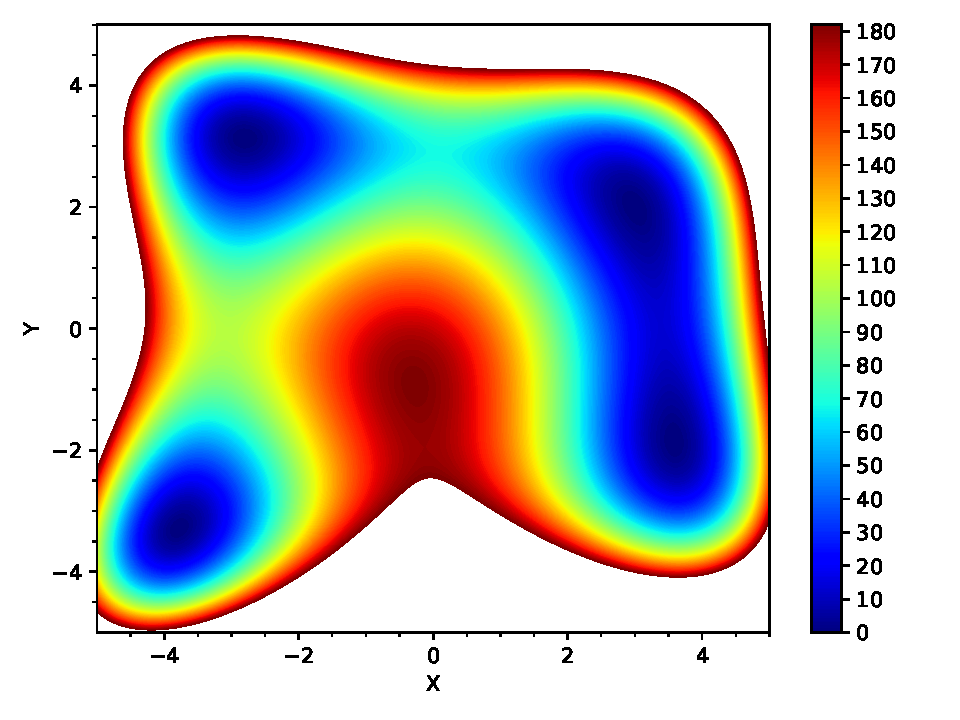
\includegraphics[width=\textwidth]{./pics/contour2}
\caption{Контурный график функции $f\left(x, y\right) = \left(x^2 + y - 11\right)^2 + \left(x + y^2 - 7\right)^2$}
\label{fig:contour2}
\end{figure}
\end{minipage}
\vfill
\end{frame}


\begin{frame}[fragile]{Минимизация без ограничений}
\scriptsize
Исходную функцию можно определить при помощи оператора \mintinline{python}|def|:
\vfill
\begin{minted}[fontsize=\fontsize{8pt}{8pt}]{pycon}
>>> def f(X):
...     x, y = X
...     return (x ** 2 + y - 11) ** 2 + (x + y ** 2 - 7) ** 2
...
\end{minted}
\vfill
где массив \texttt{X} распакован в именованные переменные \texttt{x} и \texttt{y}.
\vfill
Для поиска минимума воспользуемся методом \texttt{minimize} с начальным приближением $\left(x, y\right) = \left(0, 0\right)$.
\vfill
\begin{minted}[firstnumber=last]{pycon}
>>> from scipy.optimize import minimize
>>> minimize(f, (0, 0))
      fun: 1.3782267979368085e-13
 hess_inv: array([[ 0.01578229, -0.0094806 ],
       [-0.0094806 ,  0.03494937]])
      jac: array([-3.95019932e-06, -1.19075692e-06])
  message: 'Optimization terminated successfully.'
     nfev: 48
      nit: 10
     njev: 16
   status: 0
  success: True
        x: array([2.99999994, 1.99999999])
\end{minted}
\vfill
\end{frame}


\begin{frame}[fragile]{Минимизация без ограничений}
\scriptsize
Метод \texttt{minimize} возвращает объект типа словарь с информацией о минимизации.
\begin{table}[h!]
\begin{tabular}{|p{.2\textwidth}|p{.8\textwidth}|}
\hline
\textbf{Параметр} & \textbf{Значение} \\
\hline
\mintinline{python}|success| & Логическое значение, сообщающее, была минимизация успешной или нет \\
\hline
\mintinline{python}|x| & Если минимизация успешна, то содержит решение: значения $\left(x_1, x_2, \ldots, x_n\right)$, в которых найден минимум функции. Если алгоритм минимизации завершился неудачно, то \texttt{x} содержит точку аварийного останова \\
\hline
\mintinline{python}|fun| & Если минимизация успешна, то содержит значение функции в точке минимума, определенной как \texttt{x} \\
\hline
\mintinline{python}|message| & Строка, описывающая результат минимизации \\
\hline
\mintinline{python}|jac| & Значение матрицы Якоби: если минимизация успешна, то значения в этом массиве должны быть близкими к нулю \\
\hline
\mintinline{python}|hess, hess_inv| & Матрица Гессе и обратная ей матрица (если использовалась) \\
\hline
\mintinline{python}|nfev, njev, nhev| & Количество операций вычисления анализируемой функции, ее якобиана и гессиана \\
\hline
\end{tabular}
\end{table}
\vfill
\end{frame}


\begin{frame}[fragile]{Минимизация без ограничений}
\scriptsize
Некоторые из методов оптимизации, используемые методом \texttt{scipy.optimize.minimize}:
\begin{table}[h!]
\begin{tabular}{|p{.2\textwidth}|p{.8\textwidth}|}
\hline
\textbf{Метод} & \textbf{Описание} \\
\hline
\mintinline{python}|BFGS| & Алгоритм BFGS (Broyden-Fletcher-Goldfarb-Shanno), принятый по умолчанию для минимизации без ограничений или граничных условий \\
\hline
\mintinline{python}|Nelder-Mead| & Алгоритм Нелдера–Мида, также известный как симплекс-метод (спуска) или
метод деформируемого многогранника (амебы). Не требует производных \\
\hline
\mintinline{python}|CG| & Метод сопряженных градиентов \\
\hline
\mintinline{python}|Powell| & Ломано-линейный алгоритм в доверительной области (неограниченная минимизация). Требуются матрицы Якоби и Гессе (которые обязательно должны быть положительно определенными) \\
\hline
\mintinline{python}|TNC| & Усеченный алгоритм Ньютона для минимизации с граничными условиями \\
\hline
\mintinline{python}|l-bfgs-b| & Минимизация с ограничениями и граничными условиями с использованием алгоритма L-BFGS-B \\
\hline
\mintinline{python}|slsqp| & Метод минимизации <<последовательное программирование методом наименьших квадратов>> (sequential least-squares programming) с граничными условиями и ограничениями по равенству и неравенству \\
\hline
\end{tabular}
\end{table}
\vfill
Алгоритм, используемый \texttt{minimize}, определяется с помощью передаваеймой в аргументе строки \texttt{method} строки. Алгоритм, применяемый по умолчанию~-- BFGS.
\vfill
\end{frame}


\begin{frame}[fragile]{Минимизация без ограничений}
\scriptsize
Найдем максимум функции $f\left(x, y\right) = \left(x^2 + y - 11\right)^2 + \left(x + y^2 - 7\right)^2$ при помощи алгоритма BFGS, для этого минимизируем функцию $-f\left(x, y\right)$:
\vfill
\begin{minted}{pycon}
>>> from scipy.optimize import minimize
>>> def f(X):
...     x, y = X
...     return (x ** 2 + y - 11) ** 2 + (x + y ** 2 - 7) ** 2
...
>>> minimize(lambda X: -f(X), (-.2, -1))
      fun: -181.61652152258267
 hess_inv: array([[ 0.02312334, -0.0065379 ],
       [-0.0065379 ,  0.06119262]])
      jac: array([0., 0.])
  message: 'Optimization terminated successfully.'
     nfev: 24
      nit: 5
     njev: 8
   status: 0
  success: True
        x: array([-0.27084461, -0.9230386 ])
\end{minted}
\vfill
\end{frame}

\subsection{Минимизация с ограничениями}
\begin{frame}[fragile]{Минимизация с ограничениями}
\scriptsize
\begin{itemize}
\item Иногда необходимо найти максимум или минимум объекта функции с одним или несколькими ограничениями. Чтобы воспользоваться описанным выше методом в качестве примера, можно попытаться найти один минимум функции $f(x,y)$, который удовлетворяет условию $x > 0$, $y > 0$, или значение минимума функции на прямой $x = y$.
\item Алгоритмы \texttt{l-bfgs-b}, \texttt{tnc} и \texttt{slsqp} поддерживают аргумент \texttt{bounds} для передачи в метод \texttt{minimize}.
\item Значение аргумента \texttt{bounds}~-- это последовательность
кортежей, каждый из которых содержит пары (\texttt{min}, \texttt{max}) для каждой переменной функции, определяющие границы минимизации для соответствующей переменной.
\item Если в каком-либо направлении не существует ограничений, то используется значение \mintinline{python}|None|.
\end{itemize}
\vfill
\end{frame}


\begin{frame}[fragile]{Минимизация с ограничениями}
\scriptsize
Например, если выполняется попытка найти минимум функции $f\left(x, y\right) = \left(x^2 + y - 11\right)^2 + \left(x + y^2 - 7\right)^2$, начиная с $\left(−1/2, −1/2\right)$ без определения каких-либо границ, то метод \texttt{slsqp} обеспечивает сходимость (почти точную) к минимуму в точке $(−2.805118, 3.131312)$:
\vfill
\begin{minted}{pycon}
>>> from scipy.optimize import minimize
>>> def f(X):
...     x, y = X
...     return (x ** 2 + y - 11) ** 2 + (x + y ** 2 - 7) ** 2
...
>>> minimize(f, (-.5, -.5), method='slsqp')
     fun: 4.0198726971069946e-07
     jac: array([-0.00721077,  0.00037714])
 message: 'Optimization terminated successfully'
    nfev: 36
     nit: 10
    njev: 10
  status: 0
 success: True
       x: array([-2.80522924,  3.131319  ])
\end{minted}
\vfill
\end{frame}


\begin{frame}[fragile]{Минимизация с ограничениями}
\scriptsize
Для обеспечения условий $x < 0$, $y < 0$, необходимо установить значения \texttt{bounds} без минимальных границ по $x$ и $y$ и максимальные границы $x = 0$ и $y = 0$:
\vfill
\begin{minted}[firstnumber=last]{pycon}
>>> xbounds = (None, 0)
>>> ybounds = (None, 0)
>>> bounds = (xbounds, ybounds)
>>> minimize(f, (-.5, -.5), method='slsqp', bounds=bounds)
     fun: 4.115667606325133e-08
     jac: array([-0.00283595, -0.00034243])
 message: 'Optimization terminated successfully'
    nfev: 39
     nit: 11
    njev: 11
  status: 0
 success: True
       x: array([-3.77933774, -3.28319868])
\end{minted}
\vfill
\end{frame}


\begin{frame}[fragile]{Минимизация с ограничениями}
\scriptsize
\begin{itemize}
\item Предположим, что необходимо найти точки экстремума функции $f\left(x, y\right) = \left(x^2 + y - 11\right)^2 + \left(x + y^2 - 7\right)^2$, которые также соответствуют условию x = y (т. е. лежат на диагонали графика, изображенного на рисунке~\ref{fig:contour2}).
\item Ограничения определяются как аргумент \texttt{constraints} для метода \texttt{minimize} в виде словаря, определяющего строковые ключи: \mintinline{python}|'type'|~-- тип ограничения и \mintinline{python}|'fun'|~-- вызываемый объект, реализующий это ограничение.
\item Значением \mintinline{python}|'type'| может быть \mintinline{python}|'eq'| или \mintinline{python}|'ineq'| для ограничения, основанного на равенстве (например, $x = y$) или на неравенстве (например, $x > 2y - 1$).
\item Функция ограничения, основанного на равенстве, должна возвращать ноль, если ограничение соблюдено, а функция ограничения, основанного на неравенстве, должна возвращать неотрицательное значение, если ограничение соблюдено.
\end{itemize}
\vfill
\end{frame}


\begin{frame}[fragile]{Минимизация с ограничениями}
\scriptsize
Для поиска минимума функции $f(x, y)$ с ограничением $x = y$ можно воспользоваться методом \texttt{slsqp} с функцией ограничения, основанного на равенстве, возвращающей $x - y$.
\vfill
\begin{minted}[firstnumber=last]{pycon}
>>> constr = {'type': 'eq', 'fun': lambda X: X[0] - X[1]}
>>> minimize(f, (0, 0), method='slsqp', constraints=constr)
     fun: 8.000000000716087
     jac: array([-16.33084416,  16.33130538])
 message: 'Optimization terminated successfully'
    nfev: 25
     nit: 7
    njev: 7
  status: 0
 success: True
       x: array([2.54138438, 2.54138438])
\end{minted}
\vfill
\end{frame}


\subsection{Минимизация функции одной переменной}
\begin{frame}[fragile]{Минимизация функции одной переменной}
\scriptsize
\begin{itemize}
\item В том случае когда оптимизируемая функция зависит только от одной переменной, можно использовать более быстрый метод \texttt{scipy.optimize.minimize\_scalar}.
\item Для быстрого определения минимума данный метод можно вызвать с аргументом \mintinline{python}|method='brent'|, определяющим использование реализации метода Брента для нахождения минимума.
\item Для данного метода желательно сначала установить интервал поиска минимума, подставив для \texttt{x} значения \texttt{(a, b, c)} такие, что $f(a) > f(b)$ и $f(c) > f(b)$. Это можно выполнить при помощи аргумента \texttt{bracket}, в который передается кортеж \texttt{(a, b, c)}.
\item Однако, если это невозможно или слишком сложно, то можно передать интервал из двух значений \texttt{x}, в котором начинается поиск минимума ограниченный области в направлении убывания функции.
\item В тех случаях, когда значение параметра \texttt{bracket} не задано, поиск минимума начинается с интервала $(0, 1)$.
\end{itemize}
\vfill
\end{frame}

\begin{frame}[fragile]{Минимизация функции одной переменной}
\scriptsize
\begin{minipage}{.4\textwidth}
На рисунке \ref{fig:figure_40} приведен пример графика полинома с двумя минимумами и одним максимумом.
\vfill
\end{minipage}
\begin{minipage}{.59\textwidth}
\begin{figure}[h!]
	\centering
	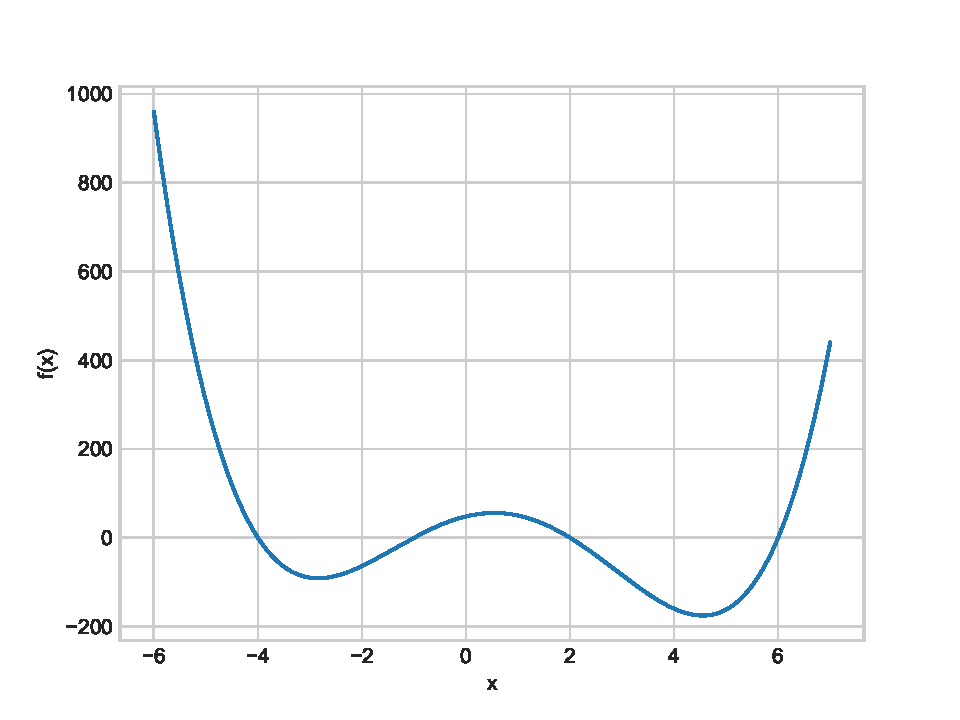
\includegraphics[width=\linewidth]{./pics/Figure_40}
	\caption{График полинома $f(x) = x^4 - 3x^3 - 24x^2 + 28x + 48$}
	\label{fig:figure_40}
\end{figure}
\end{minipage}
\vfill
\end{frame}

\begin{frame}[fragile]{Минимизация функции одной переменной}
\scriptsize
Если не указывать значения аргумента \texttt{bracket} метод \mintinline{python}|minimize_scalar| определяет минимум функции в точке $-2.841$.
\vfill
\begin{minted}{pycon}
>>> from scipy.optimize import minimize_scalar
>>> import numpy as np
>>> p = np.polynomial.Polynomial((48., 28., -24., -3., 1.))
>>> minimize_scalar(p)
     fun: -91.32163915433344
    nfev: 15
     nit: 10
 success: True
       x: -2.841044326595826
\end{minted}
\vfill
Если задать ограниченную область поиска второго минимума, передав значения $(a, b, c) = (3, 4, 6)$, соответствующие условию $f(a) > f(b) < f(c)$, то метод определит минимум функции в точке $4.549$:
\vfill
\begin{minted}[firstnumber=last]{pycon}
>>> minimize_scalar(p, bracket=(3, 4, 6))
     fun: -175.45563549487974
    nfev: 14
     nit: 10
 success: True
       x: 4.549468364257193
\end{minted}
\vfill
\end{frame}


\begin{frame}[fragile]{Минимизация функции одной переменной}
\scriptsize
Для поиска максимума методу \mintinline{python}|minimize_scalar| передается функция $-f(x)$. В этом случае область поиска минимума функции $-f(x)$ ограничивается парой значений $(-1, 0)$:
\vfill
\begin{minted}[firstnumber=last]{pycon}
>>> minimize_scalar(-p, bracket=(-1, 0))
     fun: -55.734305899213226
    nfev: 12
     nit: 8
 success: True
       x: 0.5415759589734416
\end{minted}
\vfill
\end{frame}

\section{Минимизация функций \\ нескольких переменных}
\sectionframe

\begin{frame}[fragile]{Минимизация функций нескольких переменных}
\scriptsize
\begin{itemize}
	\item Конечная цель моделирования химико-технологического процесса заключается в его более эффективной реализации или \textit{оптимизации}.

	\item \textit{Оптимизация}~-- это комплекс целенаправленных действий, заключающихся в получении наилучших результатов (значений параметров объектов) при соответствующих результатах.

	\item Оптимизация заключается в нахождении точки экстремума рассматриваемой функции или оптимальных технологических условий процесса. Для того, чтобы оценить оптимум, нужно выбрать \textit{критерий оптимизации}. \textit{Критерий оптимизации (оптимальности)}~-- это количественная оценка оптимизируемого показателя качества объекта, т.е. главный признак эффективности решения оптимизационной задачи.

	\item В зависимости от решаемой задачи, в качестве критерия оптимальности может быть выбран \textit{технологический критерий} (к примеру, максимальная селективность или выход продукта) или \textit{экономический критерий} (скажем, минимальные затраты на производство продукта при заданной производительности).

	\item Основываясь на выбранном критерии оптимальности строится \textit{целевая функция}, выражающая зависимость критерия оптимальности от входных параметров системы:
	\begin{equation}\label{obj-func}
		F = f(x_1, x_2, \ldots, x_n)
	\end{equation}
	Таким образом, точка оптимума~-- это экстремум функции~\eqref{obj-func}, а задача оптимизации сводится к нахождению этого экстремума.
\end{itemize}
\vfill
\end{frame}


\subsection{Метод Нелдера-Мида}

\begin{frame}[fragile]{Метод Нелдера-Мида}
\scriptsize
Метод Нелдера-Мида представляет собой безусловный метод оптимизации функции нескольких переменных, не требующий вычисления градиентов.
\begin{itemize}
	\item Сущность данного метода заключается в последовательном перемещении и деформации симплекса в окрестности точки экстремума посредством выполнения трех операций:

\begin{enumerate}
	\scriptsize
	\item Отражение;
	\item Растяжение;
	\item Сжатие.
\end{enumerate}

	\item Симплекс является геометрической фигурой, представляющей $n$-мерное обобщение треугольника. То есть в случае одномерного пространства~-- это отрезок; в случае двумерного пространства~-- треугольник; для трехмерного пространства~-- тетраэдр.
	\item Данный метод осуществляет поиск локальных экстремумов и может остановиться на одном из них, поэтому в случае необходимости найти глобальный экстремум функции нужно пробовать задавать другой начальный симплекс.
\end{itemize}
Метод Нелдера-Мида  имеет следующие параметры:
\begin{itemize}
	\item коэффициент отражения $\alpha > 0$, как правило, выбирается значение $1$;
	\item коэффициент сжатия $\beta > 0$, как правило, выбирается значение $0.5$;
	\item коэффициент растяжения $\gamma > 0$, как правило, выбирается значение $2$.
\end{itemize}
\vfill
\end{frame}

\begin{frame}[fragile]{Метод Нелдера-Мида}
\scriptsize
Рассмотрим минимизацию функции от $n$ переменных без ограничений. $p_0, p_1, \ldots, p_n$~-- это $(n+1)$ точки в n-мерном пространстве, определяющие текущий симплекс. Обозначим $y_i$ значения функции при значениях $p_i$ и определим:
\begin{itemize}
	\item индекс $high$, при котором $y_{high}=max\left(y_i\right)$;
	\item индекс $low$, при котором $y_{low}=min\left(y_i\right)$.
\end{itemize}
Далее определим $p_c$, как центр всех точек при условии $i \ne high$. На каждом этапе процесса $p_{high}$ заменяется новой точкой; используются три операции~-- \textit{отражение}, \textit{сжатие} и \textit{расширение}. Данные операции определяются следующим образом: отражение $p_{high}$ обозначается $p_r$ и его координаты определяются соотношением:
\begin{equation}\label{eq:reflection}
	p_r = \left(1 + \alpha\right)\cdot p_c - \alpha \cdot p_{high}
\end{equation}
\noindent где $\alpha$~-- положительная константа, коэффициент отражения.
Если $y_r$ лежит между $y_{high}$ и $y_{low}$, то $p_{high}$ заменяется на $p_r$ и мы начинаем с начала с новым симплексом.

Если $y_r < y_{low}$, т.е. если отражение произвело новый минимум, тогда мы расширяем $p_r$ до $p_e$, применяя соотношение:
\begin{equation}\label{eq:expantion}
	p_e = \gamma \cdot p_r + \left(1 - \gamma\right)\cdot p_c
\end{equation}
Коэффициент расширения $\gamma$ имеет значение больше единицы. Если $y_e < y_{low}$, то $p_{high}$ заменяется на $p_e$ и процесс начинается с начала, но если $y_e > y_{low}$, то расширение было неудачным, заменяем $p_{high}$ на $p_r$ перед возвратом в начало цикла.
\vfill
\end{frame}

\begin{frame}[fragile]{Метод Нелдера-Мида}
\scriptsize
Если после отражения $p$ на $p_r$ $y_r > y_{low}$ для всех $i \ne high$, т.е. эта замена $p$ на $p_r$ оставляет $y_r$ максимальным, тогда определяем новое значение $p_{high}$ как предыдущее значение $p_{high}$ или $p_r$ в зависимости от того, что имеет меньшее значение $y$ и определяем:
\begin{equation}\label{eq:contraction}
	p_s = \beta \cdot p_{high} + \left(1 - \beta\right) \cdot p_c
\end{equation}
Коэффициент сжатия $\beta$ лежит в диапазоне от $0$ до $1$. Далее мы принимаем $p_s$ для $p_{high}$ и переходим в начало цикла, если не выполняется условие $y_s > min\left(y_{high}, y_r\right)$, т.е. сжатая точка хуже, чем лучшая из $p_{high}$ и $p_r$. В случае такого неудачного сжатия заменяем  все $p_i$ на ${\left(p_i + p_{low}\right)}/{2}$ и повторяем процесс с начала.

Последний аспект касается критерия, используемого для выхода из цикла. В качестве такого критерия выбрана <<стандартная ошибка>> величины $y_i$ в следующем виде:
\begin{equation}\label{eq:stndard_error}
	error = \sqrt{\cfrac{\sum\limits_{i=1}^{n}\left(y_i - y_{mean}\right)^2}{n}}
\end{equation}
\noindent где $y_{mean}$~-- среднее значение.

Таким образом, величина стандартной ошибки на каждой итерации цикла сравнивается с заранее выбранной величиной, и как только значение ошибки становится меньше~-- цикл завершается. Успех такого критерия зависит от того, не станет ли симплекс слишком маленьким по отношению к кривизне поверхности до того, как будет достигнут окончательный минимум.
\vfill
\end{frame}


\begin{frame}[fragile]{Метод Нелдера-Мида}
\scriptsize
\begin{figure}[h!]
	\centering
	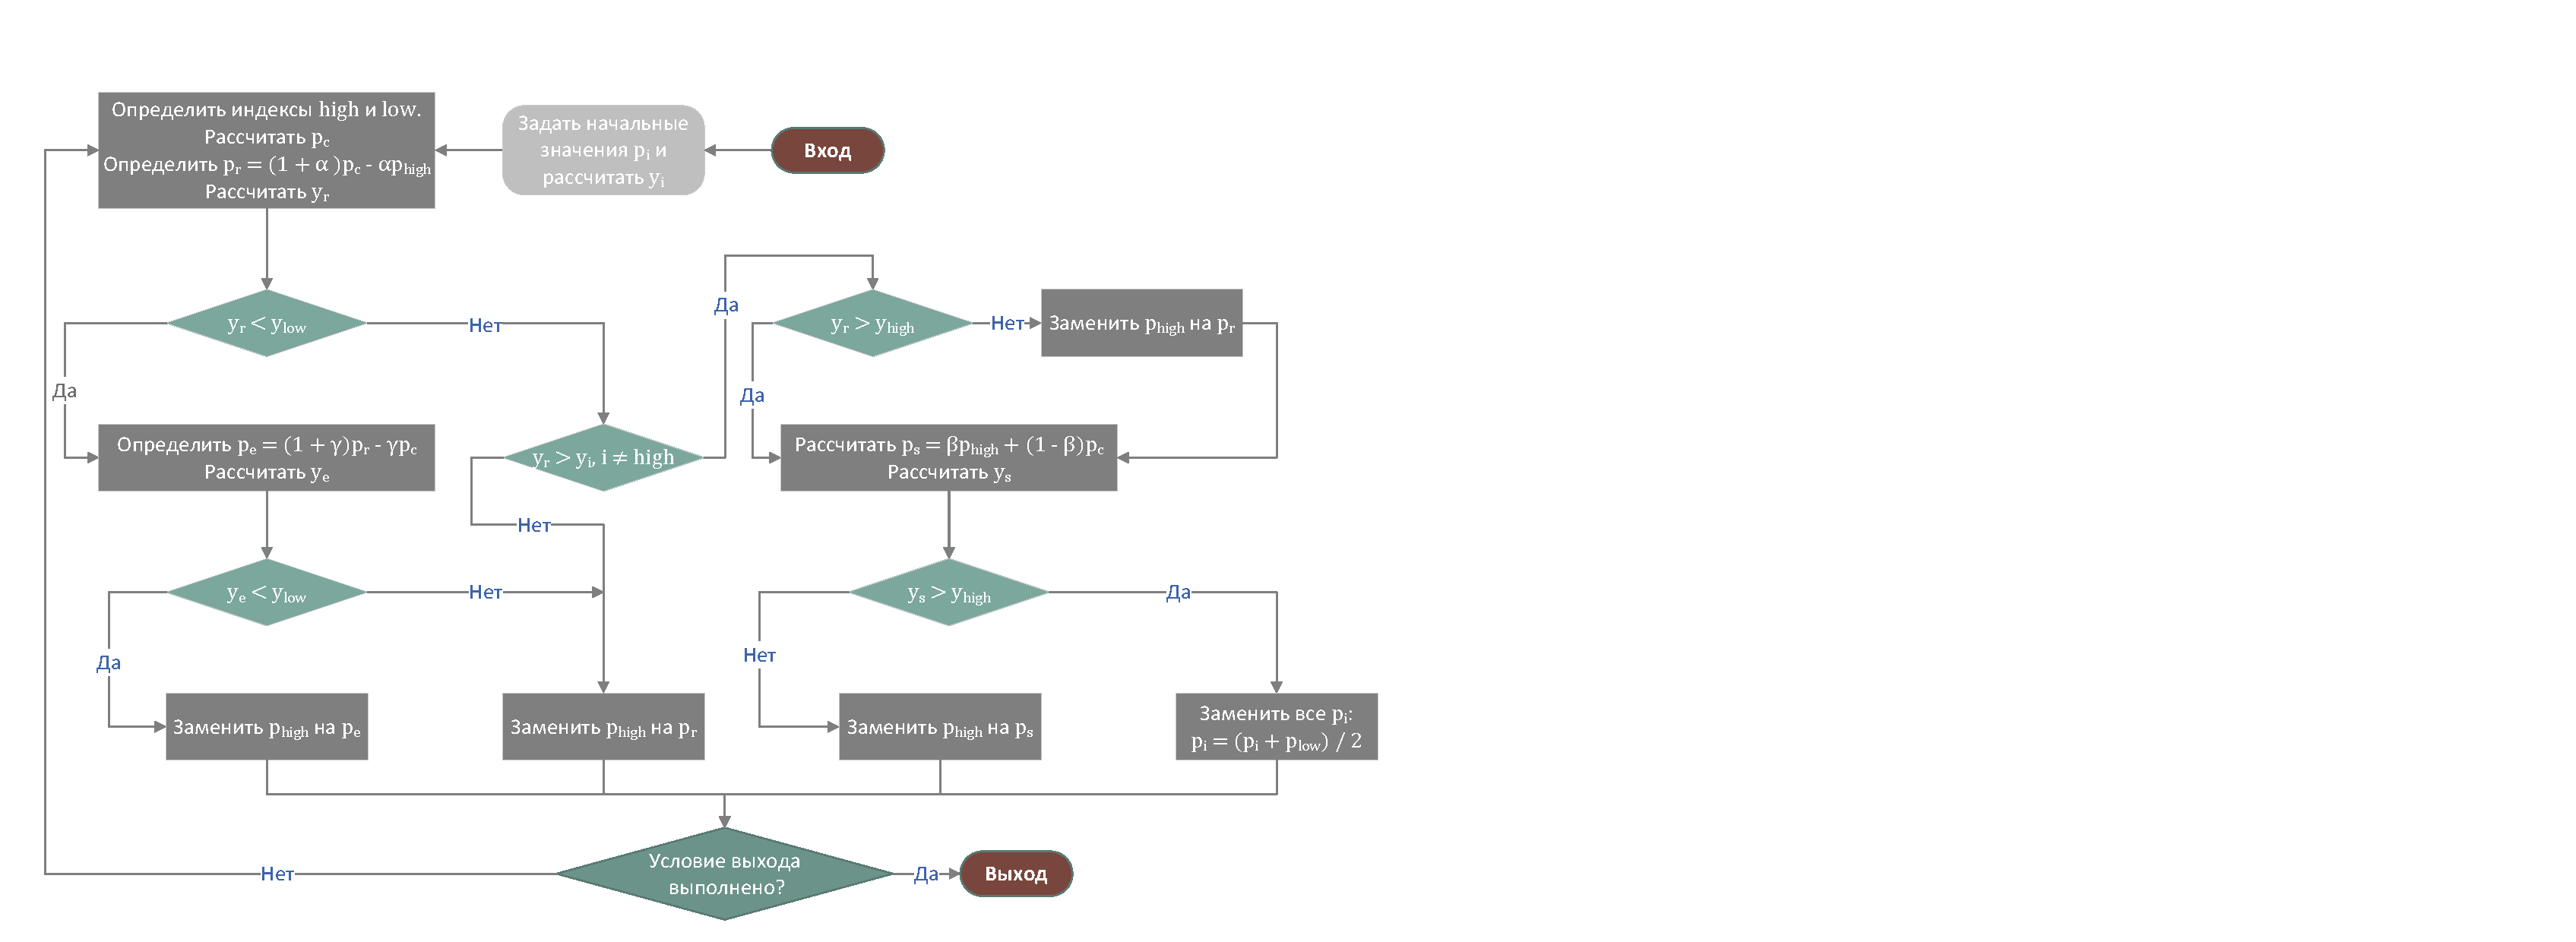
\includegraphics[width=.75\textwidth]{./pics/Nelder-Mead}
	\caption{Блок-схема алгоритма Нелдера-Мида}
	\label{fig:nelder_mead}
\end{figure}
\vfill
\end{frame}


\subsection{Пример}
\begin{frame}[fragile]{Пример}
\scriptsize
Пусть требуется найти экстремум следующей функции:
$$
f\left(x, y\right) = x^2 + xy + y^2 - 6x - 9y
$$
Из аналитического решения известно, что экстремум функции достигается в точке $f\left(1,4\right)=-21$.
\begin{figure}[h!]
	\centering
	\begin{minipage}{.45\textwidth}
		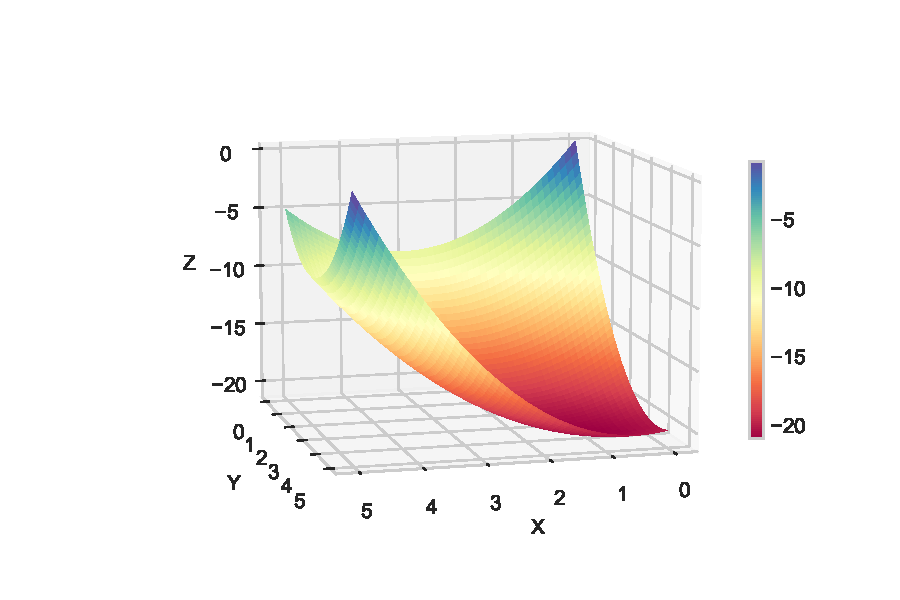
\includegraphics[width=\linewidth]{./pics/3dplot}
		\caption{3-d график функции $x^2 + xy + y^2 - 6x - 9y$}
		\label{fig:3d}
	\end{minipage}
	\begin{minipage}{.65\textheight}
		\includegraphics[width=\linewidth]{./pics/contour}
		\caption{2-d представление функции $x^2 + xy + y^2 - 6x - 9y$}
		\label{fig:contour}
	\end{minipage}
\end{figure}
Примем в качестве начального приближения следующие точки:
$
p_1\left(0,0\right); p_2\left(1,0\right); p_3\left(0, 1\right)
$
Примем в качестве критерия выхода из цикла значение стандартной ошибки равное $1\times 10^{-8}$.
\vfill
\end{frame}


\subsection{Программная реализация}
\begin{frame}[fragile]{Программная реализация}
\scriptsize
\begin{minted}{python}
def func(x):  # оптимизируемая функция
    return (x[0] ** 2 + x[0] * x[1]
            + x[1] ** 2 - 6 * x[0] - 9 * x[1])


def nelder_mead(func, initial, alpha=1, beta=0.5, gamma=2, eps=1e-8):
    """
    :param func: <function> оптимизируемая функция
    :param initial: <list-object> начальный симплекс из n+1 точек
    :param alpha: <float> коэффициент отражения; по умолчанию alpha = 1
    :param beta: <float> коэффициент сжатия; по умолчанию beta = 0.5
    :param gamma: <float> коэффициент растяжения; по умолчанию gamma = 2
    :return: <list-object> координаты точки, при которой достигается минимум функции.
    """
    n = len(initial)
    p = initial[:]
    condition = False
    y = [func(item) for item in p]
    iteration = 1
\end{minted}
\vfill
\end{frame}


\begin{frame}[fragile]{Программная реализация}
\scriptsize
\begin{minted}[firstnumber=last]{python}
    while not condition:
            high, low = y.index(max(y)), y.index(min(y))
            pc = []
            s = 0

        for j in range(n - 1):
            for i in range(n):
                if i != high:
                    s += p[i][j] / (n - 1)
            pc.append(s)
            s = 0

        pr = [(1 + alpha) * pc[i] - alpha * p[high][i] for i in range(n - 1)]  # отражение
        yr = func(pr)

        if yr < y[low]:
            pe = [(1 + gamma) * pr[i] - gamma * pc[i] for i in range(n - 1)]  # растяжение
            ye = func(pe)
            p[high] = pe[:] if ye < y[low] else pr[:]
\end{minted}
\vfill
\end{frame}

\begin{frame}[fragile]{Программная реализация}
\scriptsize
\begin{minted}[firstnumber=last]{python}
        elif all(yr > y[i] for i in range(n) if i != high):
            if yr <= y[high]:
                p[high] = pr[:]
            # сжатие
            ps = [beta * p[high][i] + (1 - beta) * pc[i] for i in range(n - 1)]
            ys = func(ps)
            if ys > y[high]:
                p = [[(p[i][j] + p[low][j]) / 2 for j in range(n - 1)] for i in range(n)]
            else:
                p[high] = ps[:]
        else:
            p[high] = pr[:]
        y = [func(item) for item in p]
        y_mean = sum(y) / n
        error = sum((y[i] - y_mean) ** 2 / n for i in range(n)) ** 0.5
        iteration += 1
        condition = error <= eps or iteration >= n * 200
    return p[low]


print(nelder_mead(func, [[0, 0], [1, 0], [0, 1]]))  # [1.0000959008633465, 3.999973542055873]
\end{minted}
\vfill
\end{frame}


\section{Генетический алгоритм}
\sectionframe


\begin{frame}[fragile]{Генетический алгоритм}
\scriptsize
\begin{itemize}
	\item Генетические алгоритмы в настоящее время широко применяются в науке и технике в качестве адаптивных алгоритмов для решения практических задач.

	\item Общепризнанно, что генетические алгоритмы особенно подходят для многомерных задач глобального поиска, где пространство поиска потенциально содержит несколько локальных минимумов. Базовый вариант генетического алгоритма не требует обширных знаний о пространстве поиска, таких как вероятные границы решения или функциональные производные.

	\item Задача, для которой простые генетические алгоритмы плохо подходят, связаны с быстрой локальной оптимизацией, однако объединение генетических алгоритмов с другими методами поиска может быть эффективным решением этой проблемы.

	\item Ярким примером задачи из области химической технологии, которую можно эффективно решить при помощи генетического алгоритма, является определение кинетических параметров химических реакций по экспериментальным данным (обратная кинетическая задача).

	\item Понятие <<генетического алгоритма>> было впервые введено Джоном Холландом для формального исследования механизмов естественной адаптации, но с тех пор данный алгоритм был адаптирован для решения задач вычислительного поиска. Современный вариант генетического алгоритма сильно отличается от первоначальной формы, предложенной Холландом.
\end{itemize}
\vfill
\end{frame}


\begin{frame}[fragile]{Генетический алгоритм}
\scriptsize
\alert{\textbf{Термины и определения}}
\begin{itemize}
	\item В природе все живые организмы содержат набор генетических данных, называемых \textcolor{extraorange}{\textit{геномом}}.
	\item Определенный набор генетической информации является \textcolor{extraorange}{\textit{генотипом}}, и точно так же определенный набор физических характеристик, или \textcolor{extraorange}{\textit{признаков}}, является \textcolor{extraorange}{\textit{фенотипом}}.
	\item Пригодность данного организма к окружающей среде обычно измеряется как его \textcolor{extraorange}{\textit{приспособленность}}. В вычислительном отношении обычно оценивают \textcolor{extraorange}{\textit{приспособленность}} организма напрямую, без учета какого-либо явления.
	\item Идея <<Выживания наиболее приспособленных>>, введенная Дарвином, хорошо известна. Там, где в природе \textcolor{extraorange}{\textit{приспособленность}} относится к способности организма выживать и размножаться, в генетических алгоритмах \textcolor{extraorange}{\textit{приспособленность}} является числовым значением некоторой \textcolor{extraorange}{\textit{целевой функции}}.
	\item Организмы с лучшим показателем \textcolor{extraorange}{\textit{приспособленности}} с большей вероятностью будут отобраны для размножения либо с помощью какого-либо механизма конкуренции за спаривание, либо в результате гибели наименее приспособленных организмов. Таким образом, гены, кодирующие полезные характеристики, передаются последующим поколениям популяции за счет генов, кодирующих вредные характеристики.
\end{itemize}
\vfill
\end{frame}


\begin{frame}[fragile]{Генетический алгоритм}
\scriptsize
\alert{\textbf{Целевые (фитнесс) функции}}
\begin{itemize}
	\item Предполагаемые решения целевой проблемы оцениваются с использованием \textcolor{extraorange}{\textit{функций приспособленности}}, так же известных как \textcolor{extraorange}{\textit{целевые функции}}.
	\item Основываясь на результатах таких функций, эволюционный процесс может быть применен к набору решений. Целевая функция будет зависеть от конкретной проблемы.
	\item Преимущество генетических алгоритмов перед многими алгоритмами поиска или оптимизации заключается в том, что не требуется определять производные целевой функции. Этот факт гарантирует, что генетический алгоритм может быть легко применен к функциям, которые содержат разрывы или другие  особенности, без каких-либо специальных обработок.
\end{itemize}
\alert{\textbf{Операторы селекции}}
\begin{itemize}
	\item Операторы селекции в генетических алгоритмах выполняют роль, эквивалентную естественному отбору. Общий эффект заключается в смещении набора генов в следующих поколениях к тем генам, которые принадлежат наиболее подходящим особям в текущем поколении.

	\item Существует множество схем отбора, описанных в литературе; выбор <<колеса рулетки>>, конкурентный выбор, случайный отбор, стохастическая выборка. Они, по сути, имитируют процессы, связанные с естественным отбором.
\end{itemize}
\vfill
\end{frame}

\begin{frame}[fragile]{Генетический алгоритм}
\scriptsize
\alert{\textbf{Оператор скрещивания}}
Существует также множество методов создания согласованного набора генов из двух родительских наборов. В данном случае скрещивание~-- это процесс, посредством которого объединяются наиболее приспособленные особи. Распространенные схемы скрещивания показаны на рисунке~\ref{fig:crossover}.
\vfill
\begin{figure}[h!]
	\centering
	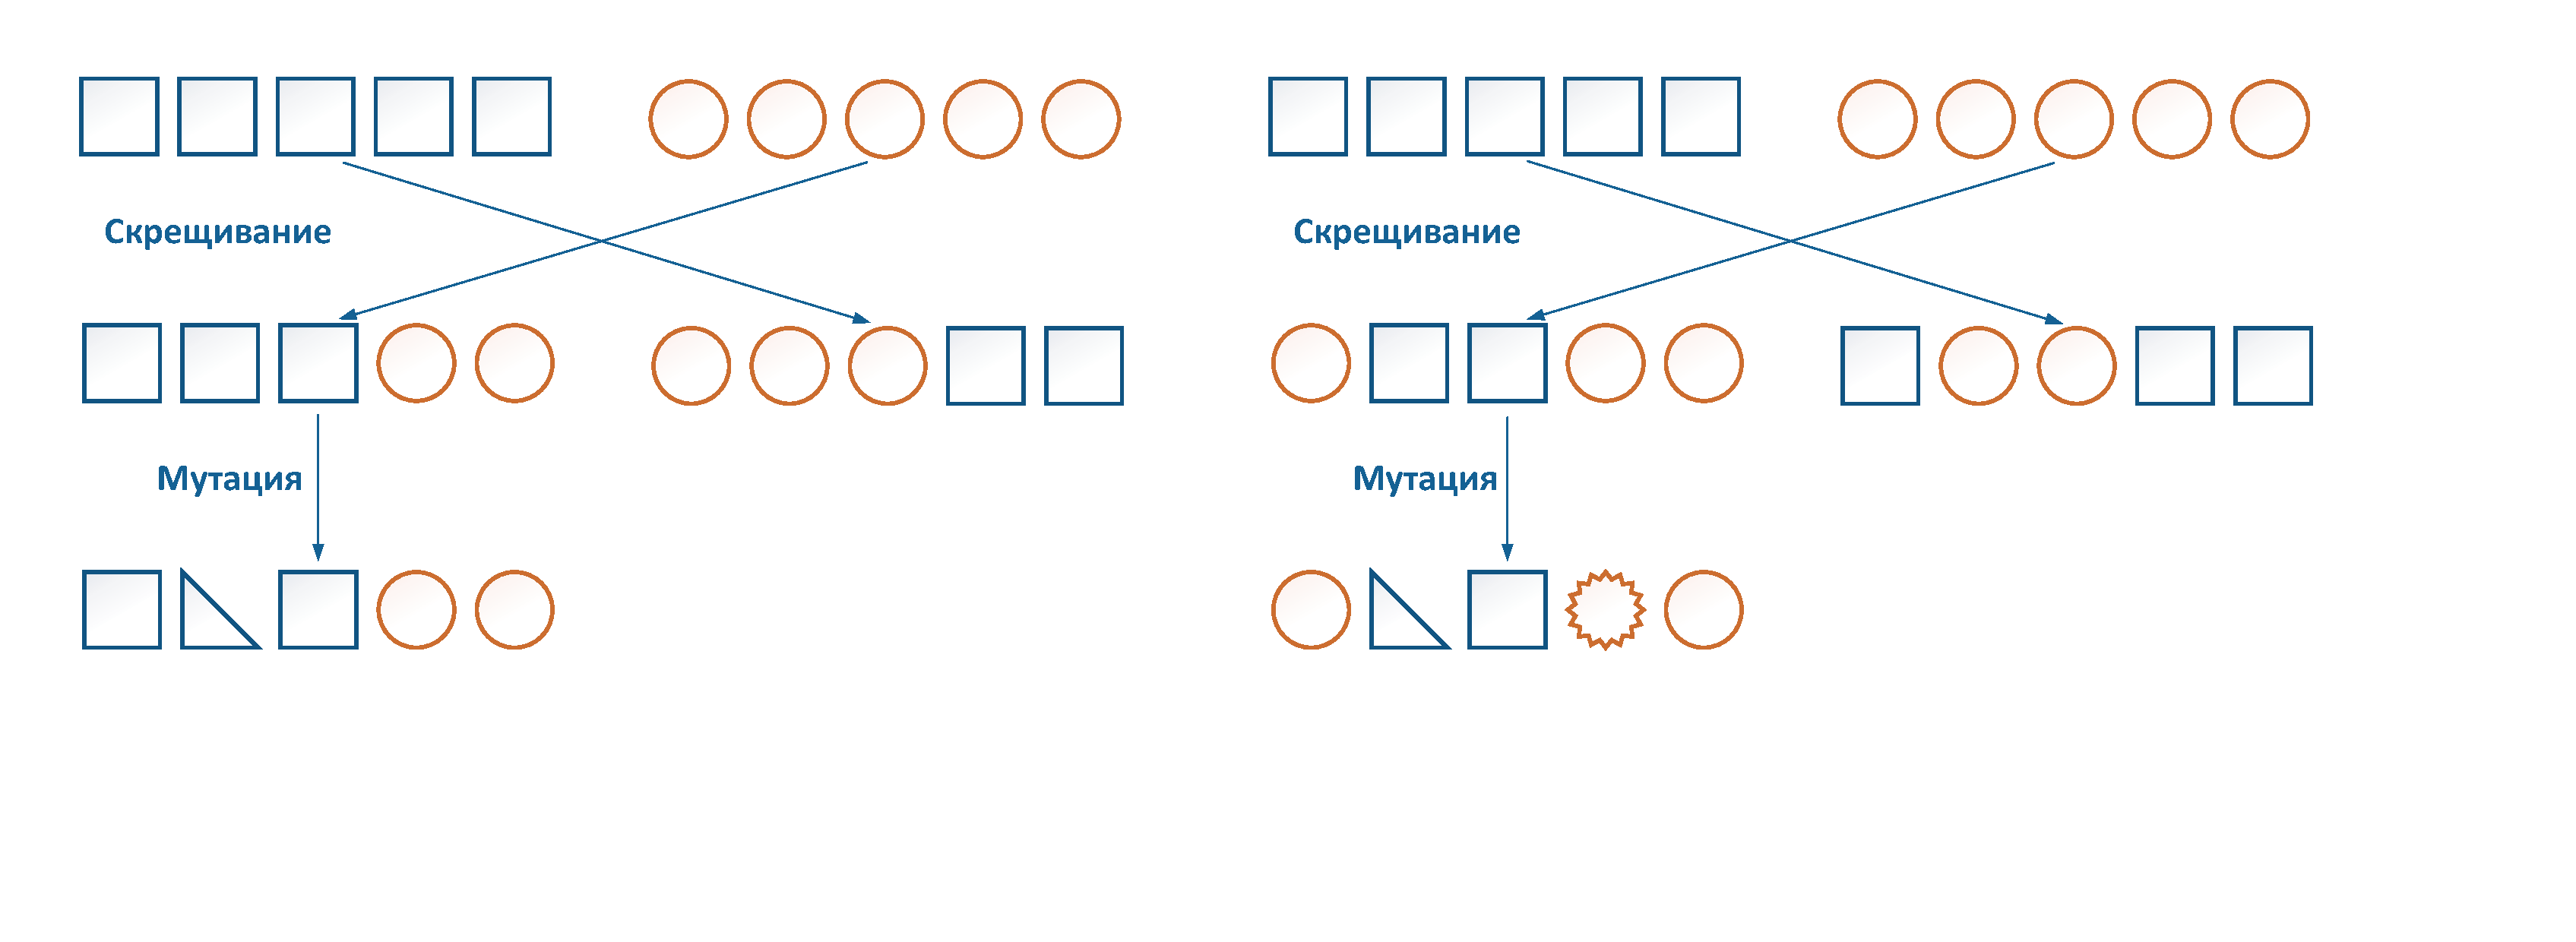
\includegraphics[width=.8\textwidth]{pics/crossover}
	\caption{Распространенные схемы скрещивания и мутации}
	\label{fig:crossover}
\end{figure}
\vfill
\alert{\textbf{Оператор мутации}}
Оператор мутации позволяют генетическому алгоритму поддерживать разнообразие, одновременно вводя некоторое поведение случайного поиска. Многие типы операторов мутации могут быть задуманы, как продолжение некоторой стратегии,  начинающейся еще при операторе скрещивания.
\vfill
\end{frame}


\begin{frame}[fragile]{Программная реализация}
\begin{minipage}{.45\textwidth}
\scriptsize
\begin{itemize}
	\item Рассмотрим один из возможных примеров реализации генетического алгоритма (рисунок~\ref{fig:ga3}).
	\item Программная реализация данного алгоритма выполнена в виде функции, при этом каждый оператор генетического алгоритма является отдельной функцией.
	\item Создание начальной популяции происходит случайным образом.
	\item  Каждый такой набор является отдельной особью (решением поставленной задачи).
	\item Совокупность таких особей и составляет популяцию.
	\item Если есть начальные приближения к решению задачи, то они добавляются к начальной популяции.
\end{itemize}
\end{minipage}
\begin{minipage}{.53\textwidth}
\begin{figure}[h!]
	\centering
	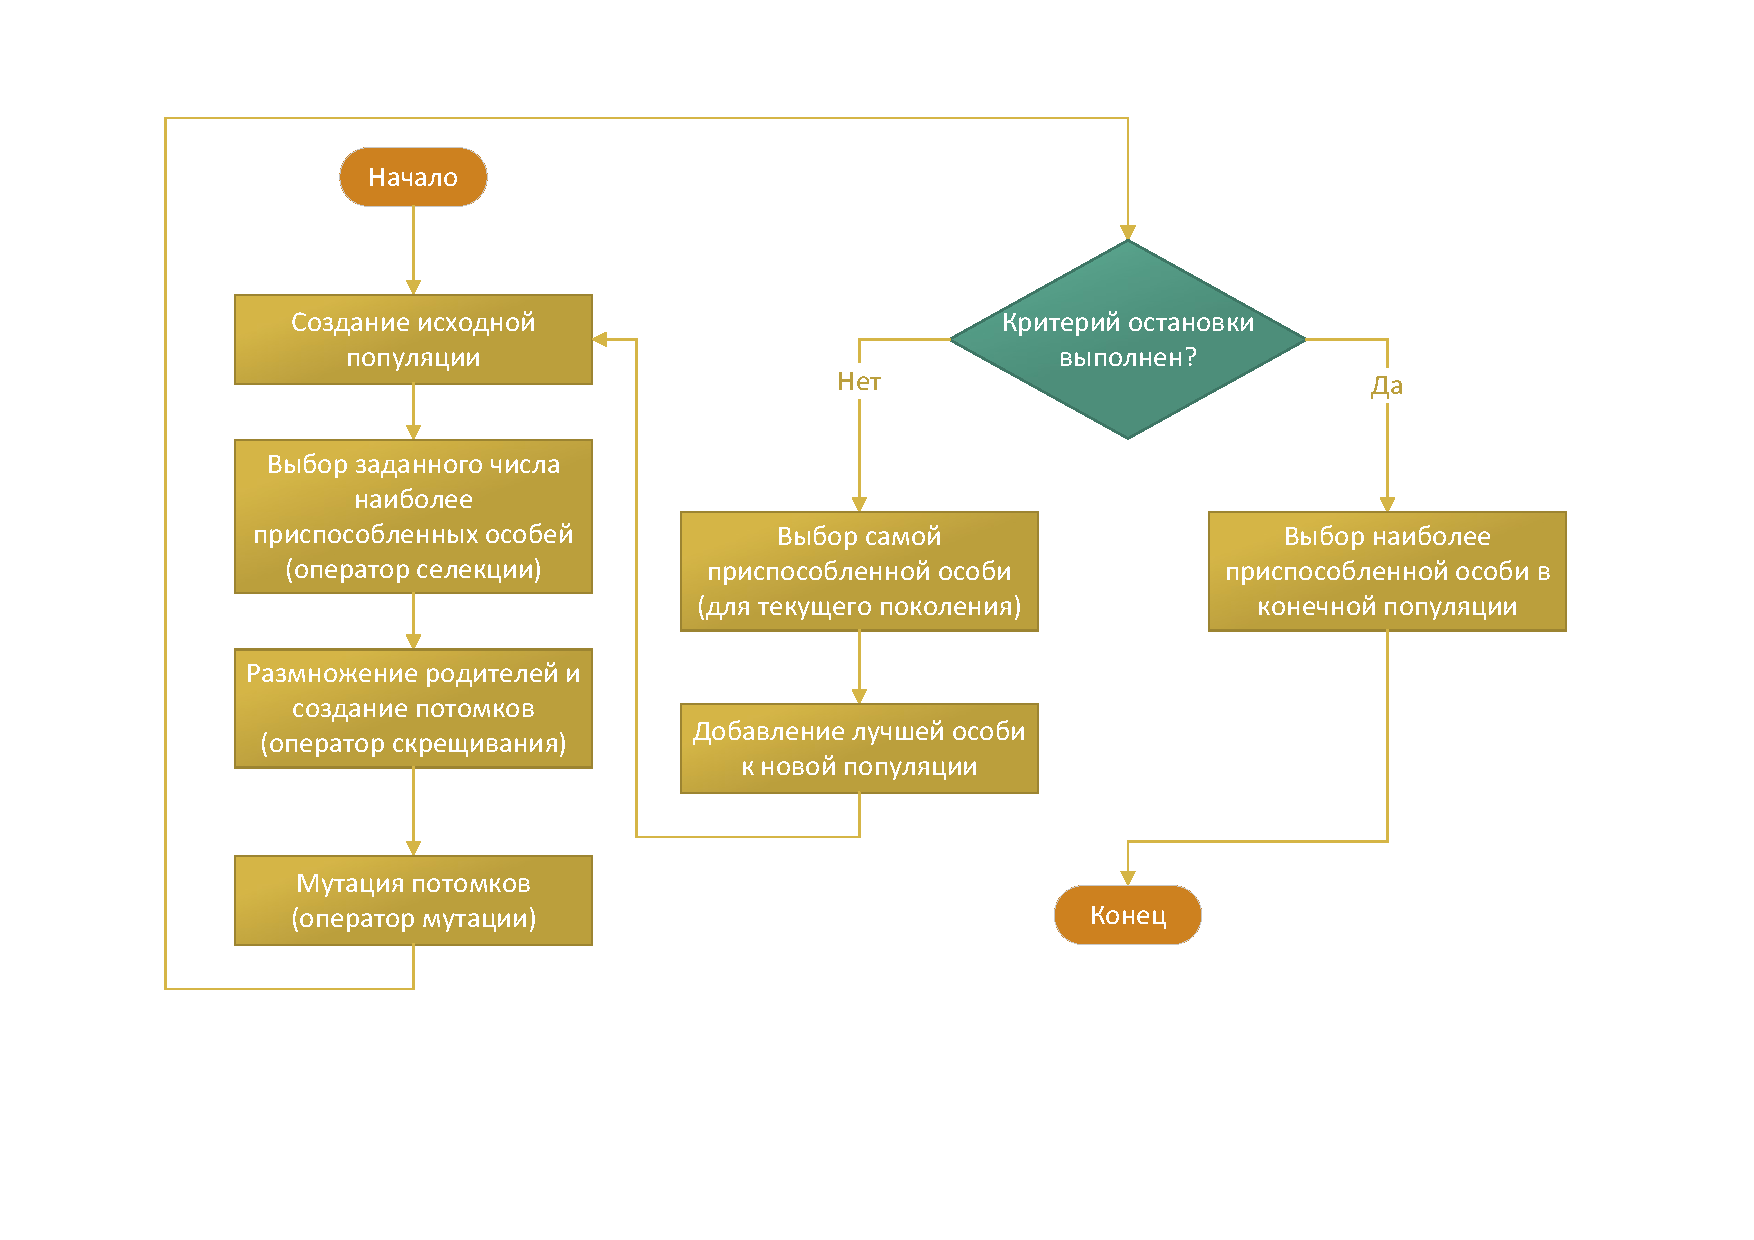
\includegraphics[width=1.15\textwidth]{pics/ga3}
	\caption{Схема генетического алгоритма}
	\label{fig:ga3}
\end{figure}
\end{minipage}
\vfill
\end{frame}

\begin{frame}[fragile]{Программная реализация}
\scriptsize
\alert{\textbf{Создание начальной популяции}}
\begin{minted}{python}
from random import uniform


def create_population(bounds, popsize, initial_guess=None):
    """
    Функция для создания исходной популяции
    :param: bounds <list-object> границы для каждого параметра в искомом решении
    :param: popsize <int-object> размер популяции
    :param: initial_guess <list-object> список начальных приближений к решению
    :return: <list-object> исходная популяция размера popsize
    """
    population = [[uniform(bounds[i][0], bounds[i][1]) for i in range(len(bounds))]
                  for _ in range(popsize)]

    if initial_guess:  # добавляем начальное приближение, если оно было введено
        return population[:-len(initial_guess)] + initial_guess
    return population
\end{minted}

После создания исходной популяции происходит сортировка всех особей по их приспособленности при помощи \textbf{оператора селекции}. Значение приспособленности для каждой особи рассчитывается при помощи целевой функции.
\vfill
\end{frame}

\begin{frame}[fragile]{Программная реализация}
\scriptsize
\alert{\textbf{Реализация оператора селекции}}
\begin{minted}{python}
def selection(func, population, selected, args):
    """
    Реализация оператора селекции
    :param: func <function-object> целевая функция, значение которой нужно оптимизировать
    :param: population <list-object> популяция особей, которые нужно отсортировать
    :param: selected <int-object> количество отобранных особей
    :param: args <tuple-object> дополнительные аргументы целевой функции (опционально)
    :return: <list-object> популяция отобранных особей размера selected
    """
    sorted_population = sorted(population, key=lambda x: func(x, *args))
    return sorted_population[:selected]
\end{minted}

На каждой итерации генетического алгоритма происходит обновление популяции созданием новых особей и уничтожения наименее приспособленных особей. Создание новых особей происходит путем моделирования процесса размножения при помощи \textbf{оператора скрещивания}. Порождающие особи называют родителями, а порожденные~-- потомками. Выбор родительских особей происходит случайным образом. При этом возможна ситуация, при которой один родитель участвует в нескольких скрещиваниях, и нет гарантированного участия в размножении всех родительских особей. Родительская пара генерирует пару потомков за счет обмена случайно выбранным набором генов.
\vfill
\end{frame}


\begin{frame}[fragile]{Программная реализация}
\scriptsize
\alert{\textbf{Реализация оператора скрещивания}}
\begin{minted}{python}
from random import randint


def crossover(selected_pop, popsize):
    """
    Реализация оператора скрещивания
    :param: selected_pop <list-object> наиболее приспособленные особи
    :param: popsize <int-object> исходный размер популяции
    :return: <list-object> популяция наиболее приспособленных особей
                           после скрещивания размера popsize
    """
    length = len(selected_pop)
    crossovered = int((popsize - length / 2)) or 1  # оператор скрещивания
                                               # выполнится хотябы один раз
    count = 0
    genome1, genome2 = [], []  # вспомогательные списки для мутирующих генов

    while count != crossovered:  # индексы выбираются случайным образом
        index1 = randint(0, length - 1)
        index2 = randint(0, length - 1)
\end{minted}
\vfill
\end{frame}

\begin{frame}[fragile]{Программная реализация}
\scriptsize
\begin{minted}{python}
        if index1 == index2:
            continue

        genome1.append(selected_pop[index1])
        genome2.append(selected_pop[index2])
        count += 1

    # граница деления генома также выбирается случайным образом
    new1 = [gen1[:(s := randint(1, len(gen1) - 1))] + gen2[s:]
            for gen1, gen2 in zip(genome1, genome2)]
    new2 = [gen1[:(s := randint(1, len(gen1) - 1))] + gen2[s:]
            for gen1, gen2 in zip(genome2, genome1)]
    new_population = selected_pop + new1 + new2

    return new_population[:popsize]
\end{minted}
Моделирование процесса мутации лучших с точки зрения приспособленности особей происходит при помощи оператора мутации, который применяется к случайным особям и изменяет случайный ген (гены) у этих особей.
\vfill
\end{frame}

\begin{frame}[fragile]{Программная реализация}
\scriptsize
\alert{\textbf{Реализация оператора мутации}}
\begin{minted}{python}
from random import uniform

def mutate(crossed_pop, limits, m_range):
    """
    Реализация оператора мутации
    :param: selected_pop <list-object> наиболее приспособленные особи
    :param: limits <list-object> пределы мутации, в которых будут изменяться гены
    :param: m_range <float-object> коэффициент затухания мутации m_range >= 1
    :return: <list-object> популяция отобранных особей размера selected
    """
    low = 1 - (1 - limits[0]) / m_range # стремится к 1 с ростом поколений
    high = 1 + (limits[1] - 1) / m_range
    length = len(crossed_pop)
    # особи для мутации выбираются случайным образом
    indexes = [randint(0, length - 1) for _ in range(length)]
    mutation_coeff = uniform(low, high)
    mutated = crossed_pop[:]
    for i in indexes:
        mutated[i] = [item * mutation_coeff for item in mutated[i]]
    return mutated
\end{minted}
\vfill
\end{frame}


\begin{frame}[fragile]{Программная реализация}
\scriptsize
\alert{\textbf{Реализация функции генетического алгоритма}}
\begin{minted}[fontsize=\fontsize{7.5pt}{8pt}]{python}
import math

def genetic_algorithm(bounds, func, initial_guess=(), args=(),
                      popsize=1000, selection_size=200, mutation_limits=(0.5, 1.2),
                      mutation_range=1, generations_count=100):
    """
    Реализация генетического алгоритма для оптимизации целевой функции
    :param: bounds <list-object> границы для каждого параметра в искомом решении
    :param: func <function-object> целевая функция, значение которой нужно оптимизировать
    :param: initial_guess <list-object> список начальных приближений к решению,
            по умолчанию пустой кортеж
    :param: args <tuple-object> дополнительные аргументы целевой функции (опционально)
    :param: popsize <int-object> размер популяции, по умолчанию popsize=1000
    :param: selection_size <int-object> количество отобранных особей,
            по умолчанию selection_size=200
    :param: mutation_limits <tuple-object> пределы мутации, в которых будут изменяться гены,
            по умолчанию mutation_limits=(0.5, 1.2)
    :param: mutation_range <float-object> коэффициент затухания мутации,
            mutation_range >= 1, увеличивается с ростом числа поколений,
            по умолчанию mutation_range=1
    :param: generations_count <int-object> количество поколений,
            по умолчанию  generations_count=100
    :return: <list-object> лучшие особи каждого поколения, отсортированные по приспособленности
    """
\end{minted}
\vfill
\end{frame}

\begin{frame}[fragile]{Программная реализация}
\scriptsize
\begin{minted}[firstnumber=last]{python}
    best = [None for _ in range(generations_count)]
    for generation in range(generations_count):
        mutation_decrease = mutation_range + math.log(1 + generation)
        population = create_population(bounds, popsize, initial_guess)
        selected = selection(func, population, selection_size, args)
        crossed = crossover(selected, popsize)
        mutated = mutate(crossed, mutation_limits, mutation_decrease)
        population = mutated[:]
        best[generation], = selection(func, population, 1, args)
        initial_guess = [best[generation]]
    return selection(func, best, generations_count, args)
\end{minted}
\vfill
\begin{itemize}
	\item Поскольку генетический алгоритм предполагает итерационный процесс, вызов генетических операторов будет происходить внутри цикла.
	\item Критерием завершения цикла выберем достижение определенного числа поколений.
	\item Для различных задач оптимальное число поколений может отличаться, однако для обеспечения высокой степени вероятности нахождения хорошего решения зададим требуемое число поколений равное $100$.
	\item Для удобства многократного использования генетического алгоритма, его реализацию следует поместить в отдельный модуль и подключать в различные проекты по мере необходимости.
\end{itemize}
\vfill
\end{frame}

\subsection{Пример}
\begin{frame}[fragile]{Пример}
\scriptsize
Пусть дана схема химических реакций:
\vfill
$$
A \overset{k_1}{\underset{k_2}{\rightleftarrows}} B
$$
\vfill
Скорость прямой реакции: $r_1 = k_1 \cdot C_A$; скорость обратной реакции:
$r_2 = k_2 \cdot C_B$; $C_A$ и $C_B$~-- концентрации компонентов $A$ и $B$.
Изменение концентрации реагирующих веществ во времени описывается следующей системой дифференциальных уравнений:
\vfill
\begin{equation*}
	\left\{
	\begin{aligned}
		\dfrac{\partial C_A}{\partial t} &= -r_1 + r_2 \\
		\dfrac{\partial C_B}{\partial t} &= r_1 - r_2
	\end{aligned}
	\right.
\end{equation*}
\vfill
Необходимо определить константы скоростей реакций: $k_1$ и $k_2$, если известно, что к моменту времени $t=1 (c)$   $C_A = 0.4513$; $C_B = 0.5487$. Начальные условия: $C_A(0) = 1$~(моль/л); $C_B(0) = 0$~(моль/л).
\vfill
\end{frame}


\begin{frame}[fragile]{Пример}
\scriptsize
\begin{itemize}
	\item Для получения более точного решения выберем метод Рунге-Кутты и предположим, что его реализация, а также реализация генетического алгоритма, сохранены в отдельных модулях под именами \texttt{solve\_ode} и  \texttt{genetic\_algorithm}, соответственно.
	\item Для того, чтобы найти константы скоростей химических реакций по данным лабораторного эксперимента при помощи генетического алгоритма потребуется составить целевую функцию, которую нужно будет минимизировать.
	\item В данном случае можно использовать сумму квадратов разности расчетных и экспериментальных значений концентраций компонентов, участвующих в химическом превращении:
\end{itemize}
\vfill
\begin{equation*}
	F = \sum\limits_{i=1}^{n}\left(C_i^{calc}-C_i^{act}\right)^2
\end{equation*}
\noindent где $C_i^{calc}$~-- расчетная концентрация $i$-го компонента; $C_i^{act}$~-- концентрация $i$-го компонента, определенная экспериментально; $n$~-- число компонентов.

Прежде всего необходимо задать систему дифференциальных уравнений в виде функции:
\vfill
\begin{minted}{python}
def equations(t, c, k):
    right_parts = [
        -k[0] * c[0] + k[1] * c[1],
        k[0] * c[0] - k[1] * c[1]
    ]
    return right_parts
\end{minted}
\vfill
\end{frame}


\subsection{Программная реализация}
\begin{frame}[fragile]{Программная реализация}
\scriptsize
\alert{\textbf{Реализация целевой функции}}
\begin{minted}[fontsize=\fontsize{8pt}{8pt}]{python}
def obj_func(k, equations, method, t, h,
             initial_composition, actual_values):
    """
    Целевая функция для минимизации генетическим алгоритмом
    :param: k <list-object> список констант скоростей химических реакций
    :param: equations <function-object> правые части дифф. уравнений
    :param: method <function-object> численный метод решения систем дифф. уравнений
    :param: t <list-object> пределы интегрирования
    :param: h <float-object> шаг интегрирования
    :param: initial_composition <list-object> начальные условия
    :param: actual_values <list-object> фактические значения концентраций из эксперимента
    :return: <float-object> квадрат суммы октлонений расчетных концентраций от эксп-ных
    """
    # решение системы ОДУ численным методом
    c = method(equations, t[0], t[-1],
               initial_composition, h, args=(k,))

    return sum((c[-1][i] - actual_values[i]) ** 2
               for i in range(len(actual_values)))
\end{minted}
\vfill
\end{frame}


\begin{frame}[fragile]{Программная реализация}
\scriptsize
Ограничим область поиска для значения констант диапазоном $[0, 1]$.
\vfill
\begin{minted}{python}
import genetic_algorithm as ga
from solve_ode import rk


def obj_func(k, equations, method, t, h, initial_composition, actual_values):
    # решение системы ОДУ численным методом
    c = method(equations, t[0], t[-1],
    initial_composition, h, args=(k,))
    return sum((c[-1][i] - actual_values[i]) ** 2
               for i in range(len(actual_values)))


actual_values = [0.4513, 0.5487]  # экспериментальные значения
k = ga.genetic_algorithm([[0, 1], [0, 1]], obj_func,
                         args=(equations, rk, [0, 1], 0.1,
                               [1, 0], actual_values))
print(k[0])  # [0.8614790508500587, 0.12043760065726794]
\end{minted}
\vfill
По аргументу \texttt{method} можно передавать различные численные методы решения систем обыкновенных дифференциальных уравнений.
\vfill
\end{frame}



\contactsframe[\Large \textbf{Благодарю за внимание!}]{

	\bigskip
	
\includegraphics[width=.05\textwidth]{pics/home} \quad Учебный корпус №2, ауд. 136 \\
	
\includegraphics[width=.05\textwidth]{pics/mail} \quad chuva@tpu.ru \\
	
\includegraphics[width=.03\textwidth]{pics/tel} \quad +7-962-782-66-15
}

\end{document}

